% Main file for Thesis plan, Traditional Format (muthesis2026, PR07284).
% PR07284 requires 6 mandatory chapters for Thesis Traditional Format.
\PassOptionsToPackage{hypertexnames=false,hyperfootnotes=false}{hyperref}
\documentclass{muthesis2026}
\thesisplan
\usepackage[numbers]{natbib}
% natbib replaces the class's thebibliography, which added REFERENCES to the
% table of contents; restore that entry.
\renewcommand{\bibsection}{\chapter*{\bibname}\addcontentsline{toc}{chapter}{\MakeUppercase{\bibname}}\markright{\bibname}}
\setcounter{secnumdepth}{3}
\usepackage{graphicx}
\graphicspath{{figures/}}
\usepackage{latexsym}
\usepackage{amsmath}
\usepackage{amsthm}
\usepackage{amssymb}
\usepackage{url}
\urlstyle{same}
\usepackage{textcomp}
\usepackage{caption,setspace}
\captionsetup{font={stretch=1.5}}
\usepackage[flushleft]{threeparttable}

\usepackage{pgfplots}
\pgfplotsset{compat=1.18}

\usepackage{booktabs}
\usepackage{array}
\usepackage{dcolumn}
\usepackage{etoolbox}
\usepackage{colortbl}
\usepackage{multirow}
\usepackage{microtype}
\usepackage{hyphenat}
\usepackage{algorithm}
\usepackage{algpseudocode}
\emergencystretch=1em

\makeatletter
% muthesis2026 sets tocdepth to 0, which also hides every entry of the lists of
% tables and figures; PR07284 No. 4.1.1.6 requires their page numbers, so list
% them at level 0.
\renewcommand*\l@figure{\@dottedtocline{0}{0em}{2.3em}}
\renewcommand*\l@table{\@dottedtocline{0}{0em}{2.3em}}
\renewcommand{\@dotsep}{10000}
% primitive \input, which is expandable, so that \hline can follow it in a tabular
\newcommand{\inputrows}[1]{\@@input #1 }
\setlength{\@fptop}{0pt}
\setlength{\@fpbot}{0pt plus 1fil}
\setlength{\@fpsep}{14pt}
\setlength{\emergencystretch}{3em}
% Table numbers: d{x.y} is a column aligned on the decimal point (x digits
% before it, y after); \best{x.y}{value} sets one cell of it in bold and \hd
% centres a header over it. dcolumn typesets numbers in math mode, so the digits
% and the point are taken from the Times text font, as in the rest of the table.
\DeclareSymbolFont{tabdigits}{OT1}{ptm}{m}{n}
\SetSymbolFont{tabdigits}{bold}{OT1}{ptm}{b}{n}
\def\tab@digit#1{\mathcode`#1=\numexpr\symtabdigits*"100+`#1\relax}
\def\tab@digits{\tab@digit0\tab@digit1\tab@digit2\tab@digit3\tab@digit4%
  \tab@digit5\tab@digit6\tab@digit7\tab@digit8\tab@digit9\tab@digit.}
\newcolumntype{d}[1]{>{\tab@digits\DC@{.}{.}{#1}}c<{\DC@end}}
\newcolumntype{B}[1]{>{\boldmath\tab@digits\DC@{.}{.}{#1}}c<{\DC@end}}
% Every table float takes its digits (and the thousands comma) from Times as
% well, in all cells and in the caption.
\AtBeginEnvironment{table}{\tab@digits\mathcode`\,=\numexpr"6000+\symtabdigits*"100+`\,\relax}
\makeatother
\newcommand{\best}[2]{\multicolumn{1}{B{#1}}{#2}}
\newcommand{\hd}[1]{\multicolumn{1}{c}{#1}}

% Approved title change (Graduate Studies Division, Nov 2026): all capitals except technical terms,
% so MLOps keeps its casing on the cover, approval pages and abstract.
\title{Enhanced Adversarial Drift Detection for \NoCaseChange{MLOps} Feature \mbox{Monitoring}}
\author{Nusrat Begum}
\hypersetup{pdftitle={Enhanced Adversarial Drift Detection for MLOps Feature Monitoring},pdfauthor={Nusrat Begum}}

\candidate{Nusrat Begum} % your name (without title)

\candidatetitle{Ms.\ } % Mr.\ Miss.\ or Ms.\

\degree{MSc} % MSc or PhD

\subject{Computer Science} % subject area

%\submissionyear{} % default is current year

%\isbn{974-04-xxxx-x}

% information for page i (advisors)

\majoradvisor{Thanapon Noraset} % name of supervisor (without title)
\majoradvisortitle{Asst.~Prof.~} % Dr.~ or Asst.~Prof.~ or Assoc.~Prof.~ or Prof.~
\majoradvisorletters{Ph.D.}
\majoradvisorsubject{Computer Science}

\coadvisor{Suppawong Tuarob}
\coadvisortitle{Assoc.~Prof.~}
\coadvisorletters{Ph.D.}
%\coadvisorstatus{Major advisor} % default is Co-advisor
\coadvisorsubject{Computer Science}

%\coadvisorII{}
%\coadvisorIItitle{}
%\coadvisorIIletters{}
%\coadvisorIIsubject{}

%\coadvisorIII{}
%\coadvisorIIItitle{}
%\coadvisorIIIletters{}
%\coadvisorIIIsubject{}

% Deans as in the official template (ICT-Mahidol/MahidolThesis, 9 Jun 2026).
% TODO (Nusrat): confirm the co-advisor, the chair and the members' academic titles.
\programchair{Assoc.~Prof.~Boonsit Yimwadsana}
\programchairqual{Ph.D.} % the class adds the program subject in parentheses
\faculty{Information and Communication Technology}
%\facultyI{} % use if faculty name is too long for one line
%\facultyII{}
\graduatestudiesdean{Prof.~Dr.~Chartchalerm Isarankura-Na-Ayudhya,\\Ph.D. (Medical Technology)}
%\GSDstatus{Acting}

% information for page ii (exam committee)

\submissiondate{December 8, 2026} % defense date

\chair{Asst.~Prof.~Akara Supratak}
\chairqual{Ph.D.}
\chairsubject{Computer Science}
\memberI{Dr.~Siripen Pongpaichet} % TODO: academic title
\memberIqual{Ph.D.}
\memberII{Dr.~Chainarong Amornbunchornvej} % TODO: academic title; NECTEC
\memberIIqual{Ph.D.}
%\memberIII{}
%\memberIIIqual{}
%\memberIV{}
%\memberIVqual{}

\facultydean{Dr.~Pattanasak Mongkolwat}
\FDqual{Ph.D.}
\FDsubject{Computer Science}
%\FDstatus{Acting}

% information for page iv (ABSTRACT)

\candidatenumber{6638009 ITCS/M}
%\major{} % major (not necessary if same as subject)
\keywords{FEATURE DRIFT DETECTION / ADVERSARIAL VALIDATION /}
\keywordsII{CLASSIFIER TWO-SAMPLE TEST / PERMUTATION TEST / MLOPS}
%\keywordsIII{}

% information for page v (THAI ABSTRACT)
% Not required for international programs (PR07284, No. 4.1.1.4).

\thaisubject{วิทยาการคอมพิวเตอร์}
\thaititle{}
\thaicandidate{}
\thaimajoradvisor{ผศ. ดร. ธนพล นรเสฏฐ์}
%\thaicoadvisor{}
%\thaicoadvisorII{}

% information for Biography

\dateofbirth{21 February 1998}
\placeofbirth{Chattogram, Bangladesh}
\firstdegreeinstitution{Stamford International University}
\firstdegreeyears{2017--2022}
\firstdegree{Bachelor of Business Administration}
\firstdegreemajor{International Business Management}
\longfirstdegree
%\preinstitution{}
%\preinstitutionLnII{}
%\preinstitutionII{}
%\preinstitutionIILnII{}
\years{2024--2026}
%\postinstitution{}
%\postinstitutionLnII{}
%\scholarship{}
%\scholarshipLnII{}
%\scholarshipLnIII{}
%\scholarshipII{}
%\scholarshipIILnII{}
%\scholarshipIILnIII{}
\position{} % present position, if applicable
\workplace{}
\workplaceLnII{}
%\homeaddress{}
%\homeaddressLnII{}
%\homeaddressLnIII{}
%\researchgrants{Grant name, funding agency, year} % TODO: add the ICT conference grant if it was awarded
%\researchgrantsLnII{}
%\researchgrantsLnIII{}
\publications{Begum N, Yamchote P, Amornbunchornvej C, Noraset T.}
\publicationsLnII{Enhanced Adversarial Drift Detection for MLOps Feature}
\publicationsLnIII{Monitoring. In: Proc. JCSSE 2026. IEEE; 2026.}
\email{nusrat.beg@student.mahidol.ac.th}


\begin{document}

\maketitle

\linespacing{1.5}
% Rewritten 23 Oct 2026. PR07284: formal language, full names with titles, at most one page.
% Nusrat: check the names and add any personal thanks (friends, funding) before submission.
\acknowledgements{
I would like to express my deepest gratitude to my major advisor, Asst.~Prof. Thanapon Noraset, Ph.D., for his guidance, patience and encouragement throughout this research. His careful reading of every draft and his questions about every result shaped how this work was designed, tested and written, and taught me to let the evidence decide what a thesis can claim.

I am sincerely grateful to my co-advisor, Assoc.~Prof. Suppawong Tuarob, Ph.D., for the advice and support given during my study, and to the chair of the thesis examination committee, Asst.~Prof. Akara Supratak, Ph.D., for the time spent reviewing this thesis and for the comments that improved it.

I thank Phaphontee Yamchote and Chainarong Amornbunchornvej, Ph.D., my co-authors on the JCSSE 2026 paper, for their contributions and discussions. I also thank the Faculty of Information and Communication Technology, Mahidol University, for the academic environment and resources that made this research possible, and my classmates and friends for their help and companionship during my study.

Finally, I owe my greatest thanks to my family for their love, patience and constant encouragement, which carried me through every stage of this degree.
}

\abstract{%
\linespacing{1.2}
Machine learning models in production can lose accuracy without warning when the distribution of their input data drifts. This thesis studies adversarial validation, in which a classifier is trained to tell reference data from recent data, as a technique for unsupervised feature drift detection. It proposes Enhanced Adversarial Drift Detection (EADD), which extends the discriminative detector D3 with a reservoir-sampled reference window, a permutation test that confirms each alarm, prediction entropy monitoring and a TreeSHAP feature ranking. Its adaptive sequential permutation test (ASPT) stops the permutation test early when the evidence is clear. EADD was compared with D3, using the same LightGBM classifier and window sizes, and with six other unsupervised detectors on thirteen real-world data streams, four of them with annotated drift points. On the annotated streams, EADD did not outperform D3: its mean recall was lower (0.50 vs.\ 0.65), its mean time to detection longer (302 vs.\ 279 samples) and its false alarms more frequent (8.9 vs.\ 5.6 per run), so the hypotheses that EADD detects more, sooner and with fewer false alarms were not supported. Most drifts that EADD missed had been signalled shortly before the annotated point. ASPT gave the same detections as a full permutation test in all runs with less runtime, and at low AUC thresholds it reduced false alarms by up to 81\% compared with EADD without a permutation test, at the cost of a lower recall (0.65 vs.\ 0.98 at a threshold of 0.3), although EADD still raised more false alarms than D3. On the streams without annotations, EADD and D3 gave almost the same classifier accuracy.
}


\tableofcontents
\listoftables
\listoffigures
\listofabbreviations{
\begin{tabbing}
\hspace{3.5cm}\=\kill
ADWIN \> Adaptive Windowing \\
ASPT \> Adaptive Sequential Permutation Test \\
AUC \> Area Under the Receiver Operating Characteristic Curve \\
BNDM \> Bayesian Nonparametric Detection Method \\
C2ST \> Classifier Two-Sample Test \\
CSDDM \> Clustered Statistical Test Drift Detection Method \\
D3 \> Discriminative Drift Detector \\
DDM \> Drift Detection Method \\
EADD \> Enhanced Adversarial Drift Detection \\
EDDM \> Early Drift Detection Method \\
FA \> False Alarms \\
$H_{\text{pred}}$ \> Prediction Entropy Monitoring Signal \\
IBDD \> Image-Based Drift Detector \\
KS \> Kolmogorov--Smirnov (test) \\
KSWIN \> Kolmogorov--Smirnov Windowing \\
LightGBM \> Light Gradient Boosting Machine \\
LPD \> Lift-per-drift \\
MD3 \> Margin Density Drift Detection \\
MLOps \> Machine Learning Operations \\
MMD \> Maximum Mean Discrepancy \\
MTD \> Mean Time to Detection \\
OCDD \> One-Class Drift Detector \\
PCA \> Principal Component Analysis \\
PSI \> Population Stability Index \\
SHAP \> SHapley Additive exPlanations \\
SPLL \> Semi-Parametric Log-Likelihood \\
TreeSHAP \> Tree-based SHAP implementation
\end{tabbing}
}


\chapter{Introduction} \label{chap:intro}

\section{Background and Significance}
Machine learning models deployed in production environments operate under the assumption that future data will resemble training data. This assumption is routinely violated: the statistical properties of input features, label distributions, or the conditional relationship between inputs and outputs evolve over time, a phenomenon usually termed \textit{concept drift} or dataset shift \citep{Lu2018, Gama2014} and referred to in this thesis as \textit{distribution drift}. Left undetected, drift degrades model performance silently, accumulating technical debt and operational risk \citep{Sculley2015, Bayram2022}. \citet{WidmerKubat1996} argued that effective learning in non-stationary environments requires detecting context changes and recovering quickly from them.

The practical consequences are well documented. \citet{Vela2022} demonstrated that standard machine learning models in four industries, including hospital operations, showed growing error as time since training increased in 91\% of 128 model-dataset pairs, even on data chosen to contain no abrupt changes. \citet{NestorEtAl2019} corroborated this finding, showing that models for common clinical tasks failed to generalise across temporally shifted patient cohorts within the same hospital system. In such settings, an alarm that only states that drift occurred leaves practitioners to work out the cause, which in production systems can lie in upstream data producers, feature pipelines or changes in the external world \citep{Sculley2015}.

The drift detection landscape has matured considerably. Statistical methods employ hypothesis tests such as the Kolmogorov--Smirnov (KS) test or Maximum Mean Discrepancy (MMD) to compare reference and current distributions \citep{Rabanser2019, Gretton2012}. Adaptive windowing methods such as Adaptive Windowing (ADWIN) dynamically adjust historical baselines \citep{BifetGavalda2007}. Supervised error-based detectors, such as the Drift Detection Method (DDM) and the Early Drift Detection Method (EDDM), monitor the model's errors (the error rate, or the distance between errors) but require ground-truth labels \citep{Gama2004, BaenaGarcia2006}. Prediction-based methods track model outputs but depend on calibration quality \citep{Sethi2017, Guo2017}. Despite this diversity, several challenges remain. Univariate tests are run once per feature, so they raise more false alarms as the number of features grows unless the significance level is corrected \citep{Rabanser2019}; supervised methods cannot operate when labels are delayed or unavailable \citep{Lu2018}; and most detectors report only when drift occurred, not how severe it is or where it occurred \citep{Lu2018}.

The discriminative approach recasts distribution comparison as a classification problem. \citet{LopezPazOquab2017} formalised this as the \textit{classifier two-sample test} (C2ST): if an auxiliary classifier can reliably separate reference from current data based solely on features, the distributions differ. In machine learning practice the same procedure is called \textit{adversarial validation} \citep{Pan2020}. This thesis studies adversarial validation as a technique for feature drift detection and uses the term C2ST when it refers to the statistical test. \citet{Gozuacik2019} adapted this principle for streaming drift detection as the Discriminative Drift Detector (D3), which is one of the three detectors recommended by the benchmark of \citet{Lukats2024} and achieved the best mean time ratio in its experiments. D3 has three practical limitations. First, it signals drift when the area under the receiver operating characteristic curve (AUC) of a logistic regression classifier exceeds a fixed threshold of 0.7, and this threshold is not calibrated as a statistical test. Second, it compares two short adjacent windows, so a slow drift that changes both windows together can go unnoticed. Third, it discards the trained classifier after computing the AUC, so it gives no indication of which features drove the alarm.

Each of these limitations has been studied separately. The C2ST comes with a significance test \citep{LopezPazOquab2017}, permutation tests calibrate such a statistic without distributional assumptions \citep{Good2005}, and sequential Monte Carlo methods reduce the number of permutations that such tests need \citep{Gandy2009}. SHapley Additive exPlanations (SHAP) \citep{Lundberg2017} has been applied to domain classifiers to rank drifted features \citep{Maggio2021} and to the explanations of deployed models to detect shifts that change model behaviour \citep{Mougan2025}. \citet{TRIPODD2024} test feature interactions for drift, but the test needs ground-truth labels and a trained model, and its cost grows with the number of feature subsets it evaluates. \citet{HDPD2024} attribute performance changes to features but need ground-truth labels, and \citet{HinderFeature2024} define feature-wise drift formally without providing a streaming detector. This thesis combines a permutation test with sequential stopping, a long-memory reference window and a feature ranking in one unsupervised streaming detector, and compares it with D3 and other unsupervised detectors on real-world data streams.

\section{Research Objectives}
The thesis proposal set the goal of investigating adversarial validation as a feature drift detection technique. The objectives of this thesis are:

\begin{enumerate}
    \item To develop Enhanced Adversarial Drift Detection (EADD), an unsupervised feature drift detector that applies adversarial validation to data streams with a long-memory reference window and a permutation test that confirms each alarm.

    \item To compare EADD with D3 and other unsupervised drift detectors on real-world data streams, in terms of recall, detection delay and false alarms on streams with annotated drift points, and of classifier accuracy and lift-per-drift on streams without them.

    \item To determine whether a sequential stopping rule makes the permutation test faster without degrading detection, and how the AUC threshold affects EADD.
\end{enumerate}

\section{Scope of the Study}
This thesis studies unsupervised detection of feature drift, that is, changes in the input distribution $P(X)$, in data streams with numerical features. Labels are not used for detection, so changes in $P(y \mid X)$ that leave $P(X)$ unchanged are outside the scope. The evaluation uses thirteen real-world data streams, eleven of them from the benchmark of \citet{Lukats2024} and two further streams, Luxembourg and Ozone, from \citet{Souza2020}: four INSECTS streams with annotated drift points \citep{Souza2020} and nine streams without annotations. EADD is compared with D3, run with the same Light Gradient Boosting Machine (LightGBM) classifier and window sizes as EADD, and with six other unsupervised detectors from the benchmark. Synthetic data streams are not used. The TreeSHAP feature ranking that EADD reports with each detection is described but its accuracy is not evaluated, and drift adaptation, such as retraining the deployed model, is not studied.

\section{Assumptions}
The study relies on the following assumptions:
\begin{enumerate}
    \item The reference window contains data from the distribution that is considered normal, so that a difference between the reference and current windows indicates drift.
    \item Under the null hypothesis of no drift, the samples in the reference and current windows are exchangeable. The permutation test is only valid under this assumption, which is violated when consecutive samples are correlated.
    \item The drift points annotated in the INSECTS streams \citep{Souza2020} mark the true changes in their distributions.
\end{enumerate}

\section{Definitions of Terms}
\begin{description}
    \item[Feature drift (covariate drift):] a change over time in the distribution of the input features $P(X)$.
    \item[Concept drift:] a change over time in the conditional distribution $P(y \mid X)$.
    \item[Classifier two-sample test (C2ST):] a test of whether two samples come from the same distribution, based on how well a classifier can tell them apart \citep{LopezPazOquab2017}.
    \item[Adversarial validation:] the practice of training a classifier to separate two data sets, such as training data and production data, and reading a high AUC as evidence that they differ \citep{Pan2020}. As a statistical test, it is a C2ST.
    \item[Reference window and current window:] the baseline sample $W_{ref}$ and the most recent sample $W_{cur}$ that a drift detector compares.
    \item[AUC:] the area under the receiver operating characteristic curve of the classifier that separates the two windows; 0.5 means the windows cannot be separated.
    \item[Permutation test:] a test that compares the observed AUC with the AUCs obtained after randomly shuffling the window labels.
    \item[Recall:] the proportion of annotated drift points that are detected within the tolerance window of 500 samples after them.
    \item[Mean time to detection (MTD):] the average number of samples between an annotated drift point and its first matching detection, where a drift point that is not detected counts as 500 samples, the length of the tolerance window.
    \item[False alarm:] a detection that is not matched to an annotated drift point, that is, a detection outside every tolerance window or a later detection inside the tolerance window of a drift point that is already matched.
    \item[Lift-per-drift:] the gain in accuracy of a classifier that is reset at every detection over a classifier trained only at the start of the stream, divided by the number of detections, as used in the benchmark of \citet{Lukats2024}.
\end{description}

\section{Research Contribution}
This thesis makes the following contributions:

\begin{enumerate}
    \item We propose EADD, an integrated framework for unsupervised feature drift detection that combines a classifier two-sample test, a reservoir-sampled reference window, prediction entropy monitoring and an adaptive sequential permutation test (ASPT), and that ranks the features behind each confirmed drift.

    \item We add a sequential stopping rule, motivated by sequential Monte Carlo tests \citep{Gandy2009}, to the permutation test of the classifier two-sample test. On four annotated real-world streams, ASPT gave the same detections as a full permutation test in all 20 runs with 25\% less runtime, and at low AUC thresholds it reduced false alarms by up to 81\% compared with no test, at the cost of a lower recall. A simulation shows that the rule raises the Type~I error of a single test from 0.045 to 0.059 at $\alpha = 0.05$.

    \item We compare EADD with D3 and six other unsupervised detectors on thirteen real-world data streams, with D3 using the same classifier and window sizes as EADD, and test the differences for statistical significance.
\end{enumerate}

\chapter{Literature Review} \label{chap:literature}


\section{Overview}
Drift detection addresses the challenge that arises when the statistical characteristics of data evolve over time in a manner that impacts the validity of a machine learning model \citep{Lu2018, Gama2014}. According to \citet{Bayram2022}, when users, environments, or the relationships between labels and features change, model accuracy can diminish. \citet{Gama2014} and \citet{Sculley2015} emphasise that drift detection identifies such modifications early, allowing practitioners to adapt, retrain, or update the model accordingly. A robust understanding of drift types and detection methods is essential for designing effective monitoring systems. Figure~\ref{fig:feature-drift} illustrates the idea behind the discriminative detectors studied in this thesis: when the reference and current distributions overlap, a classifier cannot tell their samples apart, and when the distribution shifts, it can.

\begin{figure}[!htpb]
    \centering
    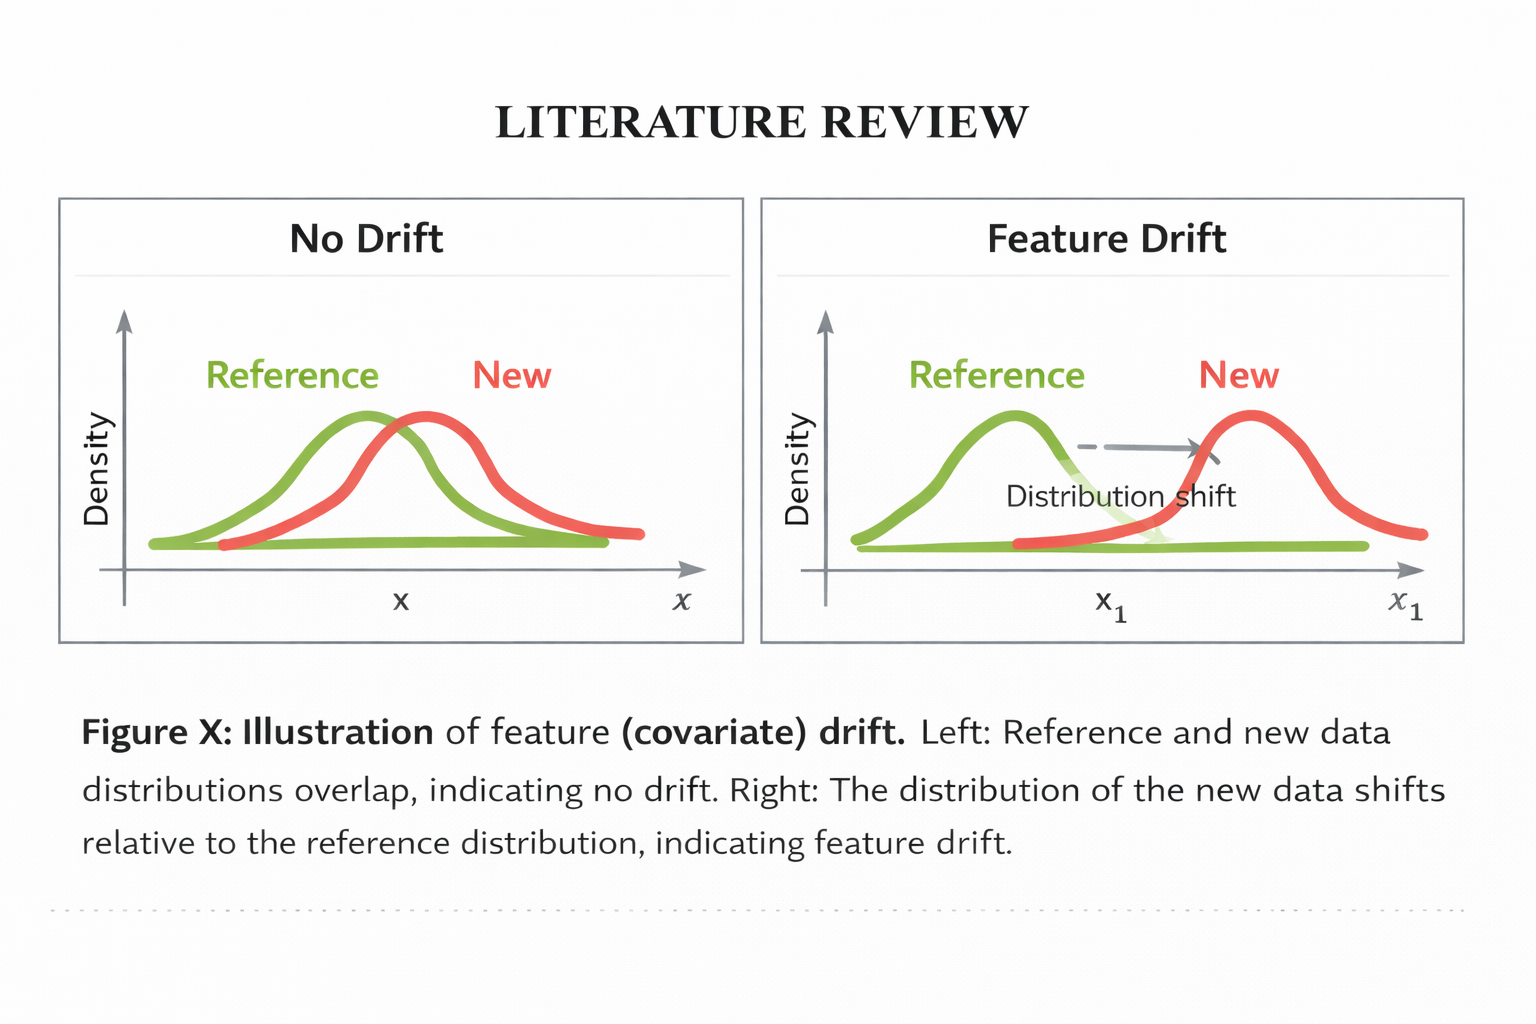
\includegraphics[width=.95\textwidth,keepaspectratio]{figures/figure-1.png}
    \caption[No drift versus drift for a discriminative classifier]{Comparison of no drift versus drift scenarios. Left: When distributions overlap, the discriminative classifier cannot distinguish data sources (AUC $\approx$ 0.5). Right: When drift occurs, distributions shift and the classifier can distinguish sources (AUC $\gg$ 0.5).}
    \label{fig:feature-drift}
\end{figure}

\section{Historical Evolution of Drift Detection}
The study of distribution drift has evolved from foundational statistical concepts to integrated AI governance over roughly seven decades. Table~\ref{tab:timeline} summarises the major eras.

\begin{table}[!htbp]
\centering
\caption[Historical evolution of drift detection research]{Historical evolution of drift detection research.}
\label{tab:timeline}
\begin{tabular}{p{3.4cm}p{10.4cm}}
\hline
\textbf{Era} & \textbf{Key Developments} \\
\hline
Early Foundations (1950s--1980s) & Statistical process control and sequential analysis laid the groundwork. \citet{Page1954} introduced the cumulative-sum (CUSUM) change-point test, which remains foundational for sequential change detection. Reservoir sampling \citep{Vitter1985} enabled representative subsampling of data streams. \\
\hline
Identification Era (1996--2004) & The term ``concept drift'', already in use since the 1980s, received an influential early treatment \citep{WidmerKubat1996}. \citet{Gama2004} introduced the Drift Detection Method (DDM), which raises warning and drift alerts when the error rate exceeds its minimum by thresholds derived from the binomial distribution, establishing the supervised error-monitoring paradigm. \\
\hline
Windowing \& Statistical Tests (2007--2015) & \citet{BifetGavalda2007} proposed ADWIN (Adaptive Windowing), enabling drift detection without fixed window sizes by applying statistical tests over dynamically adjusted sub-windows. Non-parametric tests (KS, MMD) became standard for comparing reference and current distributions \citep{Rabanser2019, Gretton2012}. \\
\hline
Deep Learning \& High-Dimensionality (2017--2023) & As models moved to unstructured data, detection shifted toward monitoring internal latent representations \citep{Rabanser2019} and toward two-sample tests on learned deep-kernel features \citep{Liu2020}. \citet{Gozuacik2019} introduced D3, demonstrating that discriminative classifiers could serve as powerful multivariate drift detectors. \citet{LopezPazOquab2017} formalised the classifier two-sample test (C2ST), providing theoretical backing for this approach. \\
\hline
Governance \& Attribution Era (2024--2026) & Attention moved toward interpretable and statistically rigorous detection: TRIPODD \citep{TRIPODD2024} introduced feature-interaction hypothesis testing; E-C2ST \citep{EC2ST2024} enabled anytime-valid sequential testing via e-values; HDPD \citep{HDPD2024} decomposed performance gaps into $P(X)$ and $P(y|X)$ components with attributions. Cloud monitoring services compare the feature attributions of production predictions (SHAP values in the case of SageMaker Clarify) with a training baseline \citep{TalySato2021, AWSSageMaker2025}. \citet{AdvAttackDrift2024} exposed vulnerabilities in discriminative detectors to adversarial evasion. \\
\hline
\end{tabular}
\end{table}

This progression, from reactive error monitoring to proactive analysis of feature distributions and attributions, provides the historical context for the present work.

\section{Types of Drift}
Drift can be categorised along two main dimensions: by the nature of the change (what component of the data-generating process is affected) and by the temporal pattern of the change (how the drift manifests over time) \citep{Lu2018, Gama2014}.

\subsection{Drift by Nature of Change}
Based on which component of the joint distribution $P(X, y)$ changes, the literature \citep{Lu2018, Gama2014, Tsymbal2004} classifies drift into the following types:

\textbf{Concept Drift (Real Drift):} The conditional distribution $P(y|X)$ changes over time while the feature distribution $P(X)$ may or may not change \citep{Lu2018, Zliobaite2010}. This represents a change in the underlying relationship between inputs and outputs: the ``concept'' the model has learned becomes invalid. For example, a news reader who has bought a house and starts looking for a holiday destination no longer finds articles on dwelling houses relevant but now finds articles on holiday homes relevant, even though the incoming articles themselves remain similar \citep{Gama2014}. Concept drift directly degrades model performance because the learned decision boundaries no longer reflect the true input-output relationship \citep{Lu2018}.

\textbf{Feature Drift (Covariate Drift):} The marginal distribution of input features $P(X)$ changes over time. When the conditional relationship $P(y|X)$ remains stable, the change is called covariate shift or virtual drift \citep{Tsymbal2004, Shimodaira2000}; a change in $P(X)$ can also accompany real concept drift. The ground-truth concept does not change, but the model may encounter inputs outside its training distribution. For example, a fraud detection model trained on transaction patterns from one demographic may receive data from a different user population, even though the definition of fraud remains unchanged. Covariate drift can degrade model performance because the model is exposed to feature regions where it may not generalise well \citep{Shimodaira2000}.

\textbf{Prior Probability Drift (Label Shift):} The marginal distribution of labels $P(y)$ changes over time while $P(X|y)$ remains stable \citep{Zliobaite2010}. This occurs when the prevalence of different classes changes, for instance a seasonal increase in a particular disease that alters the class balance in medical diagnosis. This is also called prior probability shift \citep{Lu2018}.

\textbf{Note on Terminology:} The literature uses varied terminology \citep{Lu2018}. The term ``concept drift'' is sometimes used as an umbrella term for any distribution change affecting model performance \citep{Gama2014}, while others distinguish real concept drift, a change in $P(y|X)$, from virtual concept drift, a change in the data distribution only \citep{Tsymbal2004}. This thesis focuses primarily on covariate (feature) drift detection, as it enables early warning without requiring labels.

\subsection{Drift by Temporal Pattern}
Based on how drift manifests over time, the literature \citep{Lu2018, Gama2014, Zliobaite2010} categorises drift as follows:

\begin{itemize}
    \item \textbf{Abrupt (Sudden) Drift:} A rapid, discrete change where the data distribution shifts quickly from one state to another within a short time period \citep{Gama2014}.

    \item \textbf{Gradual Drift:} A new distribution progressively replacing the old one over an extended duration, with samples from both distributions interleaved during the transition period \citep{Lu2018}.

    \item \textbf{Incremental Drift:} Small but continuous changes accumulating over time, eventually resulting in a significant distributional shift \citep{Zliobaite2010}.

    \item \textbf{Recurring (Seasonal) Drift:} Previously observed distributions reappearing after some time, often periodically due to cyclical patterns, such as seasonal effects in retail or recurring user behaviour patterns \citep{Lu2018, Gama2014}.
\end{itemize}

Understanding drift patterns is important for detector design: abrupt drift requires rapid response, gradual drift requires sustained sensitivity, and recurring drift benefits from mechanisms that can recognise previously seen distributions \citep{Gama2014}.

Figure~\ref{fig:temporal-patterns} illustrates the four patterns on a synthetic example.

\begin{figure}[!htbp]
    \centering
    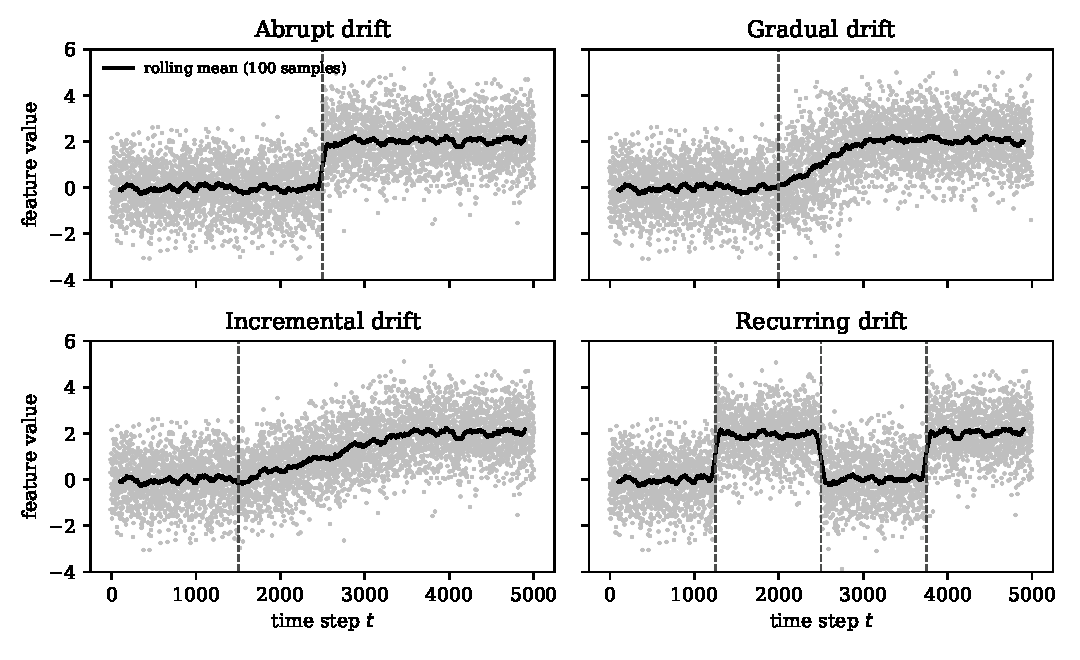
\includegraphics[width=0.95\textwidth]{figures/temporal_drift_patterns.pdf}
    \caption[Four temporal drift patterns]{The four temporal drift patterns, illustrated for one feature of a synthetic stream. Grey points are individual samples, the black line is a rolling mean over 100 samples, and dashed lines mark the drift points.}
    \label{fig:temporal-patterns}
\end{figure}

\subsection{Summary Taxonomy}
Table~\ref{tab:drift-taxonomy} consolidates the drift classification used throughout this thesis.

\begin{table}[!htbp]
\centering
\caption[Taxonomy of drift types referenced in this thesis]{Taxonomy of drift types referenced in this thesis.}
\label{tab:drift-taxonomy}
\begin{tabular}{p{2.5cm}p{3cm}p{7.6cm}}
\hline
\textbf{Category} & \textbf{Type} & \textbf{Description} \\
\hline
\multirow{3}{*}{\parbox{2.5cm}{By Cause \\ \citep{Lu2018, Gama2014}}}
  & Data / Feature Drift & Change in the input distribution $P(X)$, with or without a change in the relationship to the target. \\
  & Concept Drift & Change in the conditional $P(y \mid X)$, invalidating learned decision boundaries. \\
  & Prior Probability Drift & Change in the label distribution $P(y)$ while $P(X \mid y)$ is stable. \\
\hline
\multirow{4}{*}{\parbox{2.5cm}{By Pattern \\ \citep{Gama2014, Zliobaite2010}}}
  & Sudden (Abrupt) & Rapid, discrete shift between two distinct distributions. \\
  & Gradual & Old concept progressively replaced by a new one over an extended period. \\
  & Incremental & Small, continuous changes accumulating into a significant shift. \\
  & Recurring (Seasonal) & Previously observed distributions reappearing, periodically or irregularly. \\
\hline
\end{tabular}
\end{table}

This thesis focuses primarily on \textbf{feature (covariate) drift}, that is, changes in $P(X)$, because it can be detected without ground-truth labels and provides early warning before model performance degrades.

\section{Classification of Drift Detection Methods}
Based on surveys of the concept drift literature \citep{Lu2018, Gama2014, Tsymbal2004, Hinder2024}, drift detection methods can be classified along several dimensions. According to \citet{Lu2018}, detection algorithms can be grouped by the test statistic they apply (error rate-based, data distribution-based and multiple hypothesis tests). A further distinction, used in this thesis, is based on label availability: whether the method requires access to ground-truth labels (supervised) or operates without them (unsupervised).

\subsection{Supervised Drift Detection Methods}
Supervised detectors require ground-truth labels and monitor the error stream of the deployed model \citep{Gama2014, Gama2004}. They assume that a change in error behaviour, such as a higher error rate, errors that occur closer together, or a shift in the mean of a monitored loss, indicates drift \citep{Gama2004, BaenaGarcia2006}. The methods in this group differ mainly in the statistic they track and in the bound they use to decide that a change is significant. DDM compares the error rate and its standard deviation with thresholds derived from the binomial distribution \citep{Gama2004}. EDDM tracks the distance between consecutive errors, which makes it more sensitive to gradual drift \citep{BaenaGarcia2006}. The Page--Hinkley test accumulates the deviations of the monitored signal from its mean \citep{Page1954}, and HDDM-A and HDDM-W replace distributional assumptions with Hoeffding-type bounds, using moving averages for abrupt change and weighted moving averages for gradual change \citep{FriasBlanco2015}.

Because these methods all watch the model's errors, they share the same strengths and weaknesses. Their alarms are tied directly to model performance, and their thresholds have a clear statistical meaning. However, they need labels, which are often delayed, expensive, or unavailable in production \citep{Lu2018, Sethi2017}. They also react only after drift has already degraded performance, and they cannot detect a change in $P(X)$ that has not yet affected the error rate.

\subsection{Unsupervised Drift Detection Methods}
Unsupervised drift detection methods do not require ground-truth labels and instead monitor changes in data distribution, model outputs, or internal representations \citep{Tsymbal2004, Hinder2024}. These methods enable earlier detection of distributional shifts, before performance degradation becomes observable, which makes them valuable in production environments with label delays \citep{Sethi2017}.

\subsubsection{Statistical Distribution-Based Methods}
Statistical methods compare a reference window with a current window through hypothesis tests or distance measures \citep{Rabanser2019, Raab2020, BifetGavalda2007}. They differ in what they compare. ADWIN compares the means of sub-windows of an adaptive window and shrinks the window when they differ, with guarantees on its false positive and false negative rates \citep{BifetGavalda2007}. Kolmogorov--Smirnov Windowing (KSWIN) applies the KS test to one feature at a time over sliding windows \citep{Raab2020}, and chi-squared tests play the same role for categorical or discretised features. Divergence measures such as the Kullback--Leibler divergence, the Jensen--Shannon divergence and the Hellinger distance quantify how far apart two estimated distributions are \citep{Dasu2006, DitzlerPolikar2011}, while the Maximum Mean Discrepancy (MMD) compares whole multivariate distributions through kernel embeddings \citep{Gretton2012}.

As a group, these methods are label-free: they compare unlabeled reference and current samples with a two-sample test at a chosen significance level \citep{Rabanser2019}. Most of them, however, test one feature at a time. With $d$ features this requires $d$ tests, so unless the significance level is corrected, the probability of at least one false alarm grows with $d$ \citep{Rabanser2019}, and changes in the joint distribution that leave every marginal unchanged are missed. Multivariate tests such as MMD avoid the per-feature problem, but their power depends on the choice of kernel \citep{Gretton2012}.

Table~\ref{tab:method-comparison} compares two widely used univariate methods, the Population Stability Index (PSI) \citep{Yurdakul2018} and the KS test, with the multivariate discriminative approach used in this thesis.

\begin{table}[!htbp]
\centering
\caption[Comparison of drift detection approaches]{Comparison of drift detection approaches.}
\label{tab:method-comparison}
\begin{tabular}{p{2.7cm}p{3.5cm}p{3.5cm}p{3cm}}
\hline
\textbf{Method} & \textbf{Approach} & \textbf{Strengths} & \textbf{Limitations} \\
\hline
\textbf{PSI (Population Stability Index)} & Compares binned distributions of single features; by a rule of thumb, PSI $> 0.25$ indicates significant drift \citep{Yurdakul2018} & Simple, interpretable, widely used in credit risk & Univariate only; requires binning; misses feature correlations \\
\hline
\textbf{KS Test (Kolmogorov--Smirnov)} & Non-parametric test comparing cumulative distributions per feature & No distributional assumptions; exact p-values & Univariate only; multiple testing problem with many features \\
\hline
\textbf{Discriminative Classification} & Trains classifier to distinguish old vs. new data; uses AUC as drift signal & Multivariate; captures feature interactions; single unified test & Requires classifier training; no built-in feature attribution \\
\hline
\end{tabular}
\end{table}

Because PSI and the KS test are univariate, monitoring $d$ features requires $d$ separate tests. The discriminative approach instead tests the joint distribution of all $d$ features with a single classifier.

\subsubsection{Model-Based Discriminative Methods}
Discriminative methods train an auxiliary classifier to tell reference samples from current samples \citep{LopezPazOquab2017, Pan2020}. If the classifier separates the two sets better than chance, the distributions differ. The methods in this group differ in what they read from the classifier. Domain classifiers, also called adversarial validation in industry practice, use the AUC of a decision tree, random forest, or gradient boosting model trained to separate a training set from a test set \citep{Pan2020, Qian2021}. D3 applies this idea to data streams with a logistic regression classifier and a fixed AUC threshold \citep{Gozuacik2019}, and it is one of the three detectors recommended by a recent benchmark \citep{Lukats2024}. Margin density methods such as Margin Density Drift Detection (MD3) instead track the proportion of samples that fall close to the decision boundary of a classifier \citep{Sethi2017}.

The main strength of the group is that one classifier tests all features jointly and can capture non-linear changes that marginal tests miss \citep{LopezPazOquab2017}. No labels are needed, only the window that each sample came from \citep{Pan2020}. The costs are that a classifier must be trained at every monitoring step, that the results depend on the classifier and its hyperparameters, and that a raw AUC value has no statistical calibration unless a test, such as a permutation test, is added \citep{LopezPazOquab2017}. MD3 instead sets its margin density threshold heuristically, as $\theta$ standard deviations from a reference estimated by cross-validation \citep{Sethi2017}.

\subsubsection{Representation-Based Methods}
Representation-based methods monitor learned representations rather than raw features \citep{Rabanser2019}, or learn a feature representation for the two-sample test itself \citep{Liu2020}. They apply two-sample tests such as MMD or per-dimension Kolmogorov--Smirnov tests to low-dimensional representations of the data, such as autoencoder latents or the softmax outputs of a trained classifier \citep{Rabanser2019}, or they borrow ideas from domain adaptation and transfer learning, such as matching the distributions of learned multi-layer features with MMD \citep{Long2016}. These methods suit complex, high-dimensional data such as images, where simple kernels on raw inputs have little power to separate distributions \citep{Liu2020}, but they require a representation model and are less relevant for the tabular streams studied in this thesis.

\subsubsection{Prediction-Based and Output-Based Methods}
Prediction-based methods monitor the outputs of the deployed model without checking whether they are correct \citep{Sethi2017, Rabanser2019}. They track the distribution of predicted classes or scores \citep{Rabanser2019}, or the entropy and confidence of the predictions, under the assumption that rising uncertainty indicates out-of-distribution inputs \citep{Hendrycks2017}. Their weakness is calibration: modern models, deep networks in particular, are often poorly calibrated, and under distribution shift their confidence may not change in step with their errors \citep{Guo2017, Ovadia2019}. The prediction entropy signal used in EADD (Chapter~\ref{chap:methodology}) differs from these methods because it is computed from the discriminator that separates the two windows, not from the deployed model.

\subsubsection{Unsupervised Detectors Evaluated in Recent Benchmarks}
\citet{Lukats2024} reviewed ten fully unsupervised drift detectors and evaluated seven of them on eleven real-world data streams; the other three were too slow or depended too much on chance. They also found that the size of the observed samples was one of the most influential hyperparameters. The detectors they studied can be grouped by the mechanism they use.

The discriminative group is represented by D3 \citep{Gozuacik2019}, which achieved the best mean time ratio in the benchmark but, like the other detectors, reports only that drift occurred \citep{Lukats2024}.

Clustering-based detectors summarise each window with clusters and test whether the clusters change. The Clustered Statistical Test Drift Detection Method (CSDDM) reduces dimensionality with principal component analysis (PCA), clusters the data with K-Means, and applies statistical tests to the clusters \citep{CSDDM2021}, while UCDD assigns pseudo-labels from cluster membership and monitors shifts of the cluster boundary \citep{UCDD2020}. Many CSDDM configurations achieved a higher lift-per-drift than other detectors at a similar number of detections on some streams, a metric which measures how much classifier accuracy improves per detected drift, although its best lift-per-drift values were lower than those of D3 and SPLL \citep{Lukats2024}.

Density-based detectors model the reference distribution and flag new data that fit the model poorly. The Semi-Parametric Log-Likelihood (SPLL) detector fits a semi-parametric density model and monitors the log-likelihood of new observations \citep{SPLL2013}, NN-DVI tracks changes in nearest-neighbour density \citep{NNDVI2018}, the One-Class Drift Detector (OCDD) fits a one-class SVM to the reference data and counts the samples that fall outside its boundary \citep{OCDD2021}, and the Bayesian Nonparametric Detection Method (BNDM) compares windows with a Bayesian non-parametric P\'{o}lya tree test \citep{BNDM2020}. These detectors respond well to sudden changes in density, but they are sensitive to the size of the reference sample: BNDM signalled drift periodically when it observed few samples, and many OCDD configurations showed the same periodic behaviour \citep{Lukats2024}.

A last group reduces the stream to a simpler signal. The Image-Based Drift Detector (IBDD) converts windows of numerical data into images and compares the images \citep{IBDD2021}, and UDetect, the unsupervised change detection framework of \citet{Bashir2017}, applies Shewhart control charts to the average distance of the samples in each window to their centre, computed separately for each predicted activity class. IBDD achieved the best classifier accuracy on five of the eleven streams in the benchmark because it can signal drift again immediately after a reset, but it was among the worst detectors on mean time ratio, and 45\% of the UDetect configurations detected no drift at all \citep{Lukats2024}.

Across these groups, the benchmarked detectors report whether drift occurred but not where it occurred \citep{Lukats2024}. D3 is the only discriminative detector in the benchmark, and it relies on a fixed AUC threshold rather than a calibrated test.

\subsection{Hybrid and Ensemble Methods}
Hybrid approaches combine several sources of information, such as model predictions, embeddings, operational signals and metadata, into a single context-weighted drift score. Ensemble approaches combine several base detectors, for example through simple combination rules, although simple detector ensembles have not been shown to perform better than single drift detectors \citep{Krawczyk2017}; ensembles of classifiers combined by weighted voting are a common adaptation strategy \citep{Gama2014}. These approaches inherit the label or context requirements of their components, and ensembles that rely on a fixed set of contexts can lack suitable models when new, unknown contexts emerge \citep{Krawczyk2017}.

\section{Limitations of Existing Methods}
Each group of methods has characteristic limitations. Supervised methods need timely labels and detect drift only after performance has degraded \citep{Lu2018, Sethi2017}. Statistical tests are sensitive to noise, mostly test marginal distributions, and raise more false alarms as the number of tested features grows \citep{Rabanser2019}. Prediction-based and uncertainty-based methods depend on model calibration, which is often poor under distribution shift \citep{Guo2017, Ovadia2019}, and context-aware methods assume that the relevant contexts are known in advance, so new, unknown contexts can leave them without suitable models \citep{Krawczyk2017}.

Discriminative tests avoid several of these problems. They test the joint feature distribution directly, need neither labels nor calibrated model outputs, and make no assumption about which features matter \citep{LopezPazOquab2017, Pan2020}. In streaming drift detection, however, they have mostly been used with fixed thresholds, as in D3 \citep{Gozuacik2019}.

\section{Drift Mitigation and Adaptation Strategies}
\label{sec:mitigation}
Detecting drift is only the first step; production systems must also respond to it. Drawing on \citet{Lu2018}, \citet{Gama2014} and \citet{Krawczyk2017}, we group mitigation strategies into five categories, each with distinct trade-offs:

\begin{enumerate}
    \item \textbf{Periodic Retraining:} The model is retrained on the latest data at fixed intervals (e.g., weekly or monthly) or triggered by drift alerts. This approach is operationally simple, but fixed schedules may retrain unnecessarily or react too slowly \citep{Gama2014}.

    \item \textbf{Weighted Retraining:} Old and new data are combined for retraining, but recent examples receive higher weights, so that the influence of old examples decreases gradually. This preserves long-term knowledge while prioritising current patterns \citep{Krawczyk2017}.

    \item \textbf{Ensemble Methods:} A library of models (for example, one per season or data regime) is maintained, and predictions are combined via voting, stacking, or dynamic weighting. When drift is detected, poorly performing members are discarded and new ones trained on the current distribution \citep{Krawczyk2017}.

    \item \textbf{Online / Incremental Learning:} The model is updated continuously as each new data point (or mini-batch) arrives, making it naturally adaptive to gradual and incremental drift. This is common in streaming applications such as fraud detection and recommendation systems \citep{Gama2014, Ditzler2015}.

    \item \textbf{Human-in-the-Loop:} Uncertain or drifted samples are routed to human experts for re-labelling, which feeds into the next training iteration. Active learning frameworks that label only a budgeted fraction of samples have been combined with drift adaptation \citep{Lu2018}, which matters in domains where errors carry high cost (e.g., healthcare, autonomous driving) and labelling is expensive.
\end{enumerate}

\section{Discriminative and Attribution Approaches}

\subsection{Discriminative Distribution Testing}
Discriminative approaches to distribution comparison reframe the problem as a binary classification task: a classifier is trained to predict whether each instance originates from a reference distribution or a target distribution. High discriminative performance (AUC $\gg 0.5$) indicates the distributions are statistically separable; near-random performance suggests they are indistinguishable \citep{Pan2020, Qian2021}.

\citet{Pan2020} used this approach at Uber for the MaLTA user targeting system, training a classifier to detect mismatch between training and deployment data and, while the two stayed strongly separable, removing the most drifting features before training the targeting model. \citet{Qian2021} applied discriminative testing to manage dataset shift in credit scoring. D3 \citep{Gozuacik2019} turned the idea into a streaming detector that trains logistic regression classifiers on sliding windows and signals drift when the AUC exceeds a fixed threshold of 0.7. D3 achieved the best mean time ratio in the \citet{Lukats2024} benchmark. However, D3 applies no formal significance test, so its fixed threshold has no statistical calibration.

The \textit{classifier two-sample test} (C2ST), formalised by \citet{LopezPazOquab2017}, provided theoretical foundations for the discriminative approach: under the null hypothesis the held-out accuracy of the classifier follows a binomial distribution centred on 0.5, which gives an approximate p-value and so controls the Type~I error. A permutation test over the window labels is a common alternative that also applies to statistics such as the AUC \citep{Good2005}. A permutation test with $B$ permutations retrains the classifier $B$ times for each test. Sequential Monte Carlo tests stop drawing permutations once the decision is clear, either with uniformly bounded resampling risk \citep{Gandy2009} or with an exact sequential p-value \citep{BesagClifford1991}. The approach is label-independent, model-agnostic, and makes no assumptions about which features are important. \citet{EC2ST2024} extended C2ST with anytime-valid e-values for sequential monitoring, and \citet{MCD2024} proposed Maximum Concept Discrepancy, which uses contrastive learning as an alternative to classifier-based testing for online drift detection. C2ST and E-C2ST were designed for distribution testing rather than for streaming drift detection, and neither provides a procedure for feature-level attribution of a detected shift, although \citet{LopezPazOquab2017} note that the feature importances of the classifier can show which features separate the two samples.

D3 and other C2ST-based streaming detectors usually discard the trained classifier after computing the AUC. Practitioners therefore learn whether drift occurred but receive no guidance on which features caused it, even though the classifier has learned which features separate the two windows.

\subsection{Drift Localisation}
Drift localisation asks where a drift occurs \citep{HinderLocalization2024}. The question can be posed for regions of the data space, that is, which samples are affected, or for features, that is, which input dimensions are affected. \citet{HinderLocalization2024} formalise localisation as finding the smallest region of the data space whose removal leaves no drift, and they survey the methods that address it. Most of these methods are built on local drift detection. Binning methods such as kdq-trees partition the data space and compare the samples in each cell \citep{Dasu2006}. Neighbourhood methods compare the local density around each sample, as in the local drift degree of \citet{Liu2017LDD}. Model-based methods train a probabilistic classifier to separate time periods and read the affected regions from its predictions \citep{HinderLocalization2024}.

Feature-level localisation has developed alongside this work. \citet{Kulinski2020} framed the question of which features have shifted as a set of conditional distribution tests, one per feature, and proposed parametric and non-parametric versions based on the score function of a density model. \citet{HinderFeature2024} gave formal definitions of feature-wise drift that allow detector-agnostic selection of drifting features. TRIPODD \citep{TRIPODD2024} tests feature interactions with power guarantees, but it needs ground-truth labels and a trained model, and because it considers all feature subsets it must sample feature permutations to keep the cost manageable.

Localisation methods therefore already exist for samples, regions and features. They differ in what they require: a density model \citep{Kulinski2020}, ground-truth labels and a trained model \citep{TRIPODD2024}, or batch access to the data \citep{HinderFeature2024}. A further option, discussed next, is to explain the classifier that a discriminative test has already trained.

\subsection{Feature Attribution for Drift Detection}
Feature attribution methods explain the output of a model in terms of its input features. SHAP assigns each feature its Shapley value \citep{Shapley1953} in a cooperative game whose players are the features \citep{Lundberg2017}, and TreeSHAP computes these values exactly and in polynomial time for tree ensembles \citep{LundbergInteraction2020}. Attribution has been connected to drift in two main ways.

The first way explains a domain classifier. \citet{Maggio2021} trained a classifier to separate old data from new data and ranked the features by the mean absolute SHAP value of the classifier's output. In that study, the SHAP ranking identified the corrupted features more reliably than the classifier's impurity-based feature importance. This is the same classifier that a discriminative drift detector already trains, so the ranking adds feature-level localisation at little extra cost. Its limitations come from SHAP itself: the attributions describe the classifier rather than the data-generating process. Model-based drift explanations of this kind have also been exploratory rather than causal, which limits how directly they can guide interventions \citep{CausalDrift2025}.

The second way monitors the attributions of the deployed model. \citet{LundbergInteraction2020} monitored the SHAP values of a deployed model's loss over time, which requires labels, to find problems in its data pipeline and feature drift. \citet{Mougan2025} defined explanation shift as a change in the distribution of a model's explanations between training data and new data, and showed that it can reveal shifts that change model behaviour, including changes in feature interactions that per-feature distribution tests miss. Commercial monitoring services follow the same idea: Google Vertex AI and Amazon SageMaker Clarify compare the feature attributions of production predictions with a baseline computed during training \citep{TalySato2021, AWSSageMaker2025}.

A related line of work attributes changes in model performance, rather than changes in the data distribution, to features or to parts of the data-generating process. \citet{Zhang2023Attribution} treated the distributions that make up the data-generating process as players in a cooperative game and attributed a model's performance change to them with Shapley values. HDPD decomposes a performance gap into covariate and conditional components with per-feature attributions \citep{HDPD2024}, DBShap separates virtual and real drift with Shapley values defined over distributions \citep{DBShap2024}, and XPE combines optimal transport with Shapley values to explain how feature shifts affect performance \citep{XPE2024}. HDPD and DBShap require labels on the new data, and XPE requires a trained model and labelled source data. A recent systematic review of 82 studies found that work on explaining drift lacks benchmark datasets and standardised quantitative metrics, and that 94\% of the studies assess their explanations only qualitatively or visually \citep{XAIDriftSurvey2025}.

SHAP-based ranking of the features that separate two windows has therefore been used before \citep{Maggio2021}. This thesis does not claim it as a contribution; EADD uses it as one component of the framework.

\subsection{Other Recent Directions}
Other recent work has addressed label efficiency, explanation quality and robustness. Semi-supervised and student--teacher methods reduce or remove the need for labels \citep{CDSeer2024, STUDD2022}, per-label embedding monitoring extends drift detection to unstructured data \citep{DriftLens2024}, and autoregressive error monitoring adds confidence intervals to supervised detection \citep{ADDM2022}. For explanations, SGShift characterises concept shift with generalised additive models and controls the false discovery rate with knockoffs \citep{SGShift2025}, and \citet{CausalDrift2025} argue that drift explanations need causal rather than correlational attribution to guide remediation. \citet{AdvAttackDrift2024} showed that adversarially constructed data streams can evade common drift detectors, including discriminative ones.

\section{Gap in the Literature}
The review shows that the components of a discriminative drift detector that is both calibrated and interpretable already exist, but they have not been combined in a streaming setting. A classifier two-sample test can be calibrated \citep{LopezPazOquab2017}, for example with a permutation test \citep{Good2005}, but a fixed-budget permutation test retrains the classifier many times at every alarm, and D3, which a recent benchmark recommends, uses an uncalibrated fixed threshold instead \citep{Gozuacik2019, Lukats2024}. Sequential stopping rules that bound the probability of reaching a different decision than the exact Monte Carlo test \citep{Gandy2009} have not, to our knowledge, been applied to discriminative drift detection, and e-value tests \citep{EC2ST2024} were designed for two-sample testing, including sequential testing on a stream of batches, rather than for detecting changes in a stream.

A second gap concerns how discriminative detectors are compared. A new discriminative detector usually differs from D3 in its classifier, its window sizes, and the way it maintains its reference data. A comparison that changes all of these at once cannot show which of them causes the differences in detection delay, missed drifts and false alarms. Finally, feature-level localisation methods \citep{Kulinski2020, HinderFeature2024, TRIPODD2024}, SHAP explanations of domain classifiers \citep{Maggio2021}, and domain classifiers trained on the deployed model's SHAP values \citep{Mougan2025} answer the question of which features drifted, but they are usually run separately from, and after, detection; TRIPODD combines the two but needs ground-truth labels.

This thesis addresses these gaps with EADD, an integrated framework that combines a LightGBM classifier two-sample test, a reservoir-sampled reference window, prediction entropy monitoring and an adaptive sequential permutation test, and that reports a TreeSHAP feature ranking for every confirmed drift. The evaluation compares EADD with a version of D3 that uses the same classifier and window sizes. The two detectors differ in their reference memory and decision rule, and also in how often they check the stream (every 50 against every 200 samples) and in the number of cross-validation folds (5 against 2). The stopping rules of ASPT are motivated by sequential Monte Carlo tests but do not give an exact level-$\alpha$ test (Chapter~\ref{chap:methodology}), and the TreeSHAP ranking and $H_{\text{pred}}$ are reported but not evaluated in this thesis.


\chapter{Research Methodology} \label{chap:methodology}

This chapter first presents the conceptual framework, the research questions and the hypotheses. It then describes each step of the methodology: the datasets, the EADD framework, the baseline detectors, the implementation, the evaluation metrics, and the experimental design with its statistical analysis.

\section{Conceptual Framework}
\label{sec:framework}
Figure~\ref{fig:conceptual-framework} shows the conceptual framework of this thesis. A discriminative drift detector is defined by a few design choices: the classifier that separates the reference and current windows, the sizes of the two windows, the way the reference window is maintained, and the rule that turns the classifier's AUC into a drift decision. These choices determine the detection outcomes: how many annotated drifts are found, how quickly they are found, how many false alarms are raised, and how much computation is needed. In this thesis, EADD and D3 use the same classifier and the same window sizes. They differ in their reference memory and their decision rule, and also in how often they check the stream (every 50 samples for EADD, every 200 for D3) and in the cross-validation used for the observed AUC (5-fold for EADD, 2-fold for D3).

\begin{figure}[!htpb]
    \centering
    \begin{tikzpicture}[
        box/.style={rectangle, draw=black!65, fill=gray!10, rounded corners=2pt,
                    text width=11cm, align=center, font=\small, inner xsep=7pt, inner ysep=6pt},
        arr/.style={-{Stealth[scale=0.9]}, semithick, black!70}
    ]
    \node[box] (design) {%
        \textbf{Design choices of a discriminative detector}\\[3pt]
        Classifier: LightGBM in both EADD and D3\\
        Window sizes: $N_{ref} = 500$ and $N_{cur} = 200$ in both\\
        Reference memory: sliding (D3) or reservoir-sampled (EADD)\\
        Decision rule: AUC threshold (D3) or AUC threshold and permutation test (EADD)\\
        Check interval: every 200 samples (D3) or every 50 samples (EADD)\\
        Cross-validation of the AUC: 2-fold (D3) or 5-fold (EADD)};
    \node[box, below=0.8cm of design] (outcome) {%
        \textbf{Detection outcomes}\\[3pt]
        Recall and detection delay (MTD)\\
        False alarms (FA)\\
        Runtime};
    \draw[arr] (design) -- (outcome);
    \end{tikzpicture}
    \caption[Conceptual framework]{Conceptual framework: the design choices of a discriminative drift detector determine its detection outcomes. EADD and D3 share the classifier and the window sizes.}
    \label{fig:conceptual-framework}
\end{figure}

\section{Research Questions}
\label{sec:rq}

Based on the gaps identified in Chapter~\ref{chap:literature}, this thesis investigates three research questions:

\begin{itemize}
    \item \textbf{RQ1:} Does EADD detect annotated drifts in real-world data streams more completely and sooner than D3, and does it raise fewer false alarms?

    \item \textbf{RQ2:} Does the sequential stopping rule of ASPT make the permutation test faster without degrading detection, and how does the AUC threshold affect EADD?

    \item \textbf{RQ3:} How do EADD and the other detectors behave on real-world streams without annotated drift points?
\end{itemize}

\section{Hypotheses}
\label{sec:hypotheses}

Three hypotheses are tested at $\alpha = 0.05$ with the tests described in Section~\ref{sec:stats}:

\begin{itemize}
    \item \textbf{H1 (Detection):} On the annotated streams, EADD detects drifts more completely and sooner than D3. H1a states that the recall of EADD is higher than that of D3, and H1b that the MTD of EADD is lower than that of D3.

    \item \textbf{H2 (False Alarms):} On the annotated streams, EADD raises fewer false alarms than D3. Formally, $H_0$: $\text{FA}_{\text{EADD}} \geq \text{FA}_{\text{D3}}$ versus $H_1$: $\text{FA}_{\text{EADD}} < \text{FA}_{\text{D3}}$, where FA is the number of false alarms in a run.

    \item \textbf{H3 (ASPT):} ASPT does not degrade detection and runs faster than a full permutation test. H3a states that the recall, MTD and false alarms of EADD with ASPT do not differ from those of EADD with a full permutation test, and H3b that EADD with ASPT has a lower runtime.
\end{itemize}

H1 and H2 answer RQ1, and H3 answers RQ2. RQ3 is answered descriptively, because the streams it uses have no annotated drift points to test against.

\section{Changes from the Thesis Proposal}
\label{sec:proposal-changes}

The thesis proposal planned to study adversarial validation as a feature drift detection technique, using a logistic regression or random forest classifier, a permutation test with 200 permutations, and a rule that signals drift when the AUC is at least 0.7 and the p-value is below 0.05. It asked how effective adversarial validation is for different drift types, whether it detects drift earlier than statistical and error-based methods, and how it compares with PSI, the KS test, DDM and ADWIN. This thesis keeps that goal but changes four parts of the plan.

First, the detector was developed into EADD. The classifier was changed to LightGBM, the sliding reference window to a reservoir sample, and the fixed-budget permutation test to a sequential one, and a feature ranking was added. D3 \citep{Gozuacik2019}, a published streaming detector based on the same principle, became the main baseline. It is run with the same LightGBM classifier and window sizes as EADD, so that these choices do not confound the comparison.

Second, the baselines were changed. DDM monitors the error rate of a deployed model and therefore needs labels, while PSI, the KS test and ADWIN monitor one variable at a time. Comparing them with a multivariate unsupervised detector would require choices that are not part of these methods, such as which variable to monitor and how to combine the tests for each feature. The thesis therefore compares EADD with D3 and with six fully unsupervised detectors of the \citet{Lukats2024} benchmark, which take the same multivariate input as EADD and have tested implementations. PSI and the KS test are discussed in Chapter~\ref{chap:literature}.

Third, the proposal's questions about drift types and early detection are addressed on real-world streams with annotated drift points instead of synthetic streams. Early detection is measured by the detection delay (MTD). With one stream per drift type, the per-stream results describe differences between drift types but do not test them. Comparison with error-based detectors, which need labels, is outside the scope of the thesis.

Fourth, the evaluation was changed. The proposal's experiments used a reference and a current window of 500 samples each, checked every 200 samples, and planned to report accuracy, precision, recall and F1 and to adapt the model after each detection. EADD uses 500 reference and 200 current samples checked every 50 samples, and the detectors are evaluated by recall, MTD, false alarms and runtime on the annotated streams and by classifier accuracy and lift-per-drift on the other streams. Model adaptation after a detection is outside the scope of the thesis. The proposal's research questions were reformulated as RQ1 to RQ3, with the hypotheses H1 to H3 of Section~\ref{sec:hypotheses}.

\section{Overview of the Methodology}
Figure~\ref{fig:research-methodology} summarises the methodology. First, real-world data streams with and without annotated drift points are collected (Section~\ref{sec:datasets}). Second, each stream is processed by EADD (Section~\ref{sec:eadd}) and by the baseline detectors (Section~\ref{sec:baselines}) with several random seeds. Third, the detections are compared with the annotated drift points, or used to reset a classifier on the streams without annotations, with the metrics of Section~\ref{sec:metrics}. Section~\ref{sec:design} describes the four experiments and the statistical tests.

\begin{figure}[!htpb]
    \centering
    \begin{tikzpicture}[
        node distance=0.6cm,
        stage/.style={rectangle, draw=black!65, fill=gray!10,
                      rounded corners=2pt, text width=12.5cm,
                      align=center, font=\small, inner xsep=8pt, inner ysep=6pt},
        arr/.style={-{Stealth[scale=0.85]}, semithick, black!70}
    ]
    \node[stage] (data) {%
        \textbf{1. Data Collection}\\[2pt]
        Four INSECTS streams with annotated drift points\\
        Nine real-world streams without annotations, from \citet{Lukats2024} and \citet{Souza2020}};
    \node[stage, below=of data] (detect) {%
        \textbf{2. Drift Detection}\\[2pt]
        EADD with ASPT or no test at $\tau = 0.3$ to $0.7$, and with a full permutation test at $\tau = 0.7$\\
        D3-LightGBM; BNDM, CSDDM, IBDD, OCDD, SPLL and UDetect};
    \node[stage, below=of detect] (eval) {%
        \textbf{3. Evaluation}\\[2pt]
        Recall, MTD, false alarms and runtime on the annotated streams\\
        Classifier accuracy and lift-per-drift on the other streams\\
        Mann--Whitney U and Wilcoxon signed-rank tests};
    \draw[arr] (data) -- (detect);
    \draw[arr] (detect) -- (eval);
    \end{tikzpicture}
    \caption[Overview of the research methodology]{Overview of the research methodology: data collection, drift detection with EADD and the baseline detectors, and evaluation.}
    \label{fig:research-methodology}
\end{figure}

\section{Datasets}
\label{sec:datasets}
The population of interest is numerical data streams that are monitored for feature drift without labels. The experiments use thirteen real-world streams: the eleven streams of the benchmark of \citet{Lukats2024} and two further streams, Luxembourg and Ozone, from \citet{Souza2020}. Four of them have annotated drift points and are used to measure recall, detection delay and false alarms. The other nine have no annotations and are evaluated as \citet{Lukats2024} did, through a classifier that is reset at every detection. The labels of the streams are never given to the detectors.

\textit{Annotated (known drift points):}
\begin{itemize}
    \item \textbf{INSECTS Abrupt Balanced} \citep{Souza2020}: 52,848 samples $\times$ 33 features; abrupt changes in the sensor environment (5 annotated drift points).
    \item \textbf{INSECTS Gradual Balanced} \citep{Souza2020}: 24,150 samples $\times$ 33 features; incremental changes before and after a gradual change between two temperatures (1 annotated drift point).
    \item \textbf{INSECTS Incremental-Abrupt Balanced} \citep{Souza2020}: 79,986 samples $\times$ 33 features; incremental changes separated by abrupt ones (2 annotated drift points).
    \item \textbf{INSECTS Incremental-Reoccurring Balanced} \citep{Souza2020}: 79,986 samples $\times$ 33 features; incremental changes with a reoccurring concept (2 annotated drift points).
\end{itemize}

\textit{Unannotated (no ground-truth drift points):}
\begin{itemize}
    \item \textbf{Electricity (Elec2)} \citep{Harries1999}: 45,312 samples $\times$ 8 features; electricity market prices and demand.
    \item \textbf{INSECTS Incremental Balanced} \citep{Souza2020}: 57,018 samples $\times$ 33 features.
    \item \textbf{Luxembourg} \citep{Souza2020}: 1,900 samples $\times$ 31 features (the first of the 1,901 examples of the source file was left out).
    \item \textbf{NOAA Weather} \citep{Lukats2024}: 18,159 samples $\times$ 8 features; daily weather measurements.
    \item \textbf{Outdoor Objects} \citep{Lukats2024}: 4,000 samples $\times$ 21 features; image features of objects under changing light.
    \item \textbf{Ozone} \citep{Souza2020}: 2,534 samples $\times$ 72 features; atmospheric measurements.
    \item \textbf{PokerHand} \citep{Lukats2024}: 829,201 samples $\times$ 10 features, of which the first 100,000 were used.
    \item \textbf{Powersupply} \citep{Lukats2024}: 29,928 samples $\times$ 2 features; hourly power supply.
    \item \textbf{RialtoBridge Timelapse} \citep{Lukats2024}: 82,250 samples $\times$ 27 features; image features from a webcam.
\end{itemize}

\citet{Souza2020} give the change points of the INSECTS streams, but \citet{Lukats2024} regard only INSECTS Abrupt as having exact drift positions: the Gradual, Incremental-Abrupt and Incremental-Reoccurring streams contain no stationary periods, because the temperature keeps changing between the annotated points. Some detections counted as false alarms on these three streams may therefore correspond to real changes.

\section{The EADD Framework}
\label{sec:eadd}
EADD treats feature drift ($P(X)$ shift) detection as binary classification: if a classifier can reliably distinguish reference data from current data based solely on features, the distributions have diverged \citep{LopezPazOquab2017, Gozuacik2019}. D3 \citep{Gozuacik2019} uses this principle with a fixed AUC threshold, and \citet{LopezPazOquab2017} showed how to calibrate the test through the binomial null distribution of the held-out accuracy. EADD combines these ideas with a long-memory reference window, a sequential permutation test \citep{Good2005}, and a feature ranking for each confirmed drift.

\subsection{Problem Formulation}
\label{sec:problem}
Let $\{x_t\}_{t=1}^{T}$, with $x_t \in \mathbb{R}^d$, denote a stream of feature vectors. At each monitoring point $t$, a detector compares two windows:
\begin{itemize}
    \item a reference window $W_{ref}$ of $N_{ref}$ samples, assumed to represent the baseline feature distribution $P_{ref}(X)$, and
    \item a current window $W_{cur}$ containing the $N_{cur}$ most recent samples, drawn from the current distribution $P_{cur}(X)$.
\end{itemize}
Feature drift at time $t$ means $P_{cur}(X) \neq P_{ref}(X)$. The detector therefore tests
\begin{equation}
H_0: P_{ref}(X) = P_{cur}(X) \quad \text{versus} \quad H_1: P_{ref}(X) \neq P_{cur}(X)
\label{eq:drift-test}
\end{equation}
and outputs a decision $d_t \in \{0, 1\}$, where $d_t = 1$ signals drift. In EADD, the test statistic is the cross-validated AUC, denoted $\text{AUC}_{\text{actual}}$, of a classifier $f_\theta$ trained to separate $W_{ref}$ from $W_{cur}$. The symbol $\tau$ denotes the AUC screening threshold, $\alpha$ the significance level, and $B_{\min}$ and $B_{\max}$ the minimum and maximum numbers of permutations used by the permutation test.

Figure~\ref{fig:methodology-detailed-architecture} shows the steps of EADD, and Table~\ref{tab:eadd-alignment} lists the methods each step builds on.

\begin{figure}[!htpb]
    \centering
    \begin{tikzpicture}[
        node distance=0.56cm,
        proc/.style={rectangle, draw=black!65, fill=gray!10,
                     rounded corners=2pt, text width=7.8cm, minimum height=0.95cm,
                     align=center, font=\small, inner xsep=6pt, inner ysep=5pt},
        term/.style={rectangle, draw=black!55, fill=white,
                     rounded corners=2pt, text width=7.8cm,
                     align=center, font=\small, inner xsep=7pt, inner ysep=5pt},
        dec/.style={diamond, draw=black!65, fill=white,
                    aspect=2.2, align=center, font=\small, inner sep=2pt},
        arr/.style={-{Stealth[scale=0.85]}, semithick, black!70},
        lbl/.style={font=\footnotesize, fill=white, inner sep=1pt, text=black!70}
    ]

    \node[term] (input) {\textbf{Input Data Stream} \quad $\{x_t\}_{t=1}^{T}$};

    \node[proc, below=of input] (s1) {%
        \textbf{Step 1. Adaptive Reference Windowing}\\[-1pt]
        {\footnotesize Reservoir sampling for $W_\mathrm{ref}$\,; sliding window for $W_\mathrm{cur}$}
    };

    \node[proc, below=of s1] (s2) {%
        \textbf{Step 2. Discriminative Classification (C2ST)}\\[-1pt]
        {\footnotesize LightGBM on $W_\mathrm{ref} \cup W_\mathrm{cur}$\,; monitor AUC and $H_\mathrm{pred}$}
    };

    \node[dec, below=0.72cm of s2] (dec1) {$\mathrm{AUC} \geq \tau$?};

    \node[proc, below=0.72cm of dec1] (s3) {%
        \textbf{Step 3. Statistical Significance Testing (ASPT)}\\[-1pt]
        {\footnotesize Adaptive sequential permutation test with early stopping}
    };

    \node[dec, below=0.72cm of s3] (dec2) {$p < \alpha$?};

    \node[proc, below=0.72cm of dec2] (s4) {%
        \textbf{Step 4. Feature Ranking}\\[-1pt]
        {\footnotesize TreeSHAP ranking of the features that separate the two windows}
    };

    \node[term, below=of s4] (output) {%
        \textbf{Drift Alert Output}\\[-1pt]
        {\footnotesize uncertainty ($H_\mathrm{pred}$), significance ($p$), ranked features (SHAP)}
    };

    \draw[arr] (input) -- (s1);
    \draw[arr] (s1) -- (s2);
    \draw[arr] (s2) -- (dec1);
    \draw[arr] (dec1.south) -- node[lbl, right=2pt] {Yes} (s3.north);

    \draw[arr] (s3) -- (dec2);
    \draw[arr] (dec2.south) -- node[lbl, right=2pt] {Yes} (s4.north);

    \draw[arr] (s4) -- (output);

    \end{tikzpicture}
    \caption[Architecture of EADD]{Architecture of EADD: adaptive reference windowing, discriminative classification, ASPT significance testing, and TreeSHAP feature ranking for each confirmed drift.}
    \label{fig:methodology-detailed-architecture}
\end{figure}

\begin{table}[!htbp]
\centering
\caption[EADD components and the methods they build on]{EADD components and the methods they build on.}
\label{tab:eadd-alignment}
\begin{tabular}{p{3.4cm}p{5cm}p{5cm}}
\hline
\textbf{Component} & \textbf{EADD Step} & \textbf{Based On} \\
\hline
Reference memory & Step 1: reservoir-sampled $W_{ref}$ & Reservoir sampling \citep{Vitter1985} \\
Drift statistic & Step 2: cross-validated AUC of a LightGBM classifier & C2ST \citep{LopezPazOquab2017}; D3 \citep{Gozuacik2019}; LightGBM \citep{Ke2017} \\
Uncertainty signal & Step 2b: prediction entropy $H_{\text{pred}}$ & Shannon entropy \citep{Shannon1948} \\
Statistical confirmation & Step 3: adaptive sequential permutation test & Sequential Monte Carlo tests \citep{Gandy2009} \\
Feature ranking & Step 4: TreeSHAP ranking & SHAP \citep{Lundberg2017, LundbergInteraction2020}; \citet{Maggio2021} \\
\hline
\end{tabular}
\end{table}

\subsection{Step 1: Adaptive Reference Windowing}
To detect feature drift, the current data must be compared against a stable baseline. EADD maintains two windows consistent with established methodologies \citep{BifetGavalda2007, Tsymbal2004}:

\textbf{Reference Window ($W_{ref}$):} A buffer containing $N_{ref}$ historical samples representing the stable feature distribution $P_{ref}(X)$. Unlike sliding windows, which forget older data quickly, EADD uses \textbf{reservoir sampling} \citep{Vitter1985} so that the reference represents all samples seen since the last confirmed drift, not just the most recent batches.

\textbf{Current Window ($W_{cur}$):} A buffer containing the $N_{cur}$ most recent observations representing the current feature distribution $P_{cur}(X)$. As new data arrives, older samples are discarded to maintain responsiveness to recent changes.

\textbf{Update Mechanism:} At each monitoring step:
\begin{itemize}
    \item New samples enter $W_{cur}$
    \item Oldest samples exit $W_{cur}$
    \item Reservoir sampling maintains representative $W_{ref}$
    \item Upon confirmed drift, $W_{ref}$ is replaced by the $N_{cur}$ samples of $W_{cur}$ and filled up to $N_{ref}$ with the next $N_{ref}-N_{cur}$ samples, and $W_{cur}$ is emptied and refilled, so no check is made during the next $N_{ref}$ samples
\end{itemize}

Because each new sample is appended to $W_{cur}$ and also offered to the reservoir, $W_{ref}$ can contain samples that are also in $W_{cur}$ (about $N_{cur} N_{ref}/n_{seen}$ of them, where $n_{seen}$ is the number of samples since the last reset). These samples appear in the C2ST data with both labels, which pushes the AUC below 0.5 in a stationary stream.

\citet{Lu2018} note that window size involves a trade-off: a small window better reflects the latest data distribution, while a large window provides more data. In bias-variance terms, larger windows provide more stable estimates but slower response, and smaller windows enable faster detection but higher variance.

\subsection{Step 2: Discriminative Classification}
This step implements the \textbf{classifier two-sample test} (C2ST) \citep{LopezPazOquab2017}, also referred to as ``adversarial validation'' in industry practice \citep{Pan2020}, which forms the foundation of both D3 \citep{Gozuacik2019} and EADD. The question it asks is whether a model can tell the difference between old and new data.

\textbf{Construct Binary Classification Dataset:}
\begin{itemize}
    \item Label all samples from $W_{ref}$ as class 0 (``old'' / reference)
    \item Label all samples from $W_{cur}$ as class 1 (``new'' / current)
    \item Combined dataset: $X = W_{ref} \cup W_{cur}$, $y = \{0\}^{N_{ref}} \cup \{1\}^{N_{cur}}$
\end{itemize}

\textbf{Train Discriminative Classifier:}
A binary classifier $f_\theta$ is trained to predict the data source from the features alone. EADD uses \textbf{LightGBM} \citep{Ke2017}, a gradient boosting decision tree ensemble, as the default classifier. D3 \citep{Gozuacik2019} uses logistic regression, which can only separate the windows with a linear boundary; LightGBM can also capture non-linear differences and feature interactions. D3-LightGBM, the version of D3 used in this thesis, uses the same classifier.

\textbf{Measure Discriminative Performance:}
Classifier performance is evaluated with stratified 5-fold cross-validation:
\begin{itemize}
    \item \textbf{AUC-ROC:} the primary metric, the area under the ROC curve
    \item AUC $\approx$ 0.5 or below (the samples shared by $W_{ref}$ and $W_{cur}$, Step~1, push it below 0.5 in a stationary stream): the classifier cannot distinguish $W_{ref}$ from $W_{cur}$ $\rightarrow$ \textbf{no feature drift}
    \item AUC $\gg$ 0.5: the classifier separates the windows $\rightarrow$ $P_{ref}(X) \neq P_{cur}(X)$ $\rightarrow$ \textbf{feature drift suspected}
\end{itemize}

If the AUC reaches the screening threshold $\tau$, the alarm is passed to the significance test in Step~3. The term ``adversarial'' in EADD's name refers to this C2ST setting, in which a classifier is trained to distinguish two data sources, and not to adversarial attacks in the security or robustness sense.

\subsection{Step 2b: Prediction Entropy Monitoring ($H_{\text{pred}}$)}
After training the discriminative classifier (Step~2), EADD computes the \textbf{prediction entropy} $H_{\text{pred}}$ as an early-warning signal for distributional instability. This is the binary Shannon entropy \citep{Shannon1948} of the C2ST discriminator's output probabilities, averaged over all samples:

\begin{equation}
H_{\text{pred}} = \frac{-1}{n} \sum_{i=1}^{n} \left[\hat{p}_i \ln \hat{p}_i + (1 - \hat{p}_i) \ln (1 - \hat{p}_i)\right]
\label{eq:hpred}
\end{equation}

where $\hat{p}_i$ is the out-of-fold predicted probability, from the stratified 5-fold cross-validation of Step~2, that sample $i$ belongs to the current window ($W_{cur}$), and $n = |W_{ref}| + |W_{cur}|$ is the combined sample count.

\textbf{Interpretation:}
\begin{itemize}
    \item $H_{\text{pred}}$ near its no-drift level, which is below $\ln 2$ because the windows are unbalanced (about $-\pi\ln\pi-(1-\pi)\ln(1-\pi) \approx 0.60$ for a classifier that predicts the class proportion $\pi = N_{cur}/n = 2/7$, and lower in practice because the out-of-fold predictions are more confident): the classifier cannot distinguish windows $\rightarrow$ no distributional difference
    \item $H_{\text{pred}} \rightarrow 0$: Low entropy; the classifier clearly separates windows $\rightarrow$ strong drift signal
    \item Intermediate $H_{\text{pred}}$: Subtle distributional change that may not yet reach statistical significance
\end{itemize}

\textbf{Monitoring Property:}
$H_{\text{pred}}$ is computed at every monitoring step, including steps where the AUC has not yet reached $\tau$, so it gives a continuous view of how confidently the discriminator separates the two windows. It was intended as an early-warning signal for gradual and incremental drift, but this thesis does not evaluate it as one. A quantitative evaluation, including threshold selection and the precision and recall of pre-alarm warnings, is left to future work.

\textbf{Relationship to AUC:}
$H_{\text{pred}}$ and AUC are complementary signals. AUC measures overall discriminability, while $H_{\text{pred}}$ measures the confidence distribution of individual predictions. A high AUC with low entropy indicates clear, systematic drift; a moderately elevated AUC with higher entropy may indicate localised or emerging drift affecting only a subset of samples.

\subsection{Step 3: Adaptive Sequential Permutation Test (ASPT)}
A raw AUC score (e.g., 0.65) is inconclusive, as it may reflect genuine distributional change or statistical noise. D3 \citep{Gozuacik2019} relies on a fixed threshold (AUC $> 0.7$) without a significance test. \citet{LopezPazOquab2017} proposed the classifier two-sample test (C2ST), whose significance test uses the null distribution of the held-out accuracy; a common alternative is a fixed-budget permutation test \citep{Good2005} with a predetermined number $B$ of permutations.

\textbf{The Computational Problem:} A fixed-budget permutation test (e.g., $B=50$) wastes computation when the evidence is clear. If the actual AUC is 0.95, the first few permutations already establish significance and the remaining permutations add cost without information. Conversely, if the AUC is 0.52, early permutations quickly reveal non-significance.

\textbf{Adaptive Sequential Permutation Testing:}
EADD uses an \textbf{adaptive sequential permutation test} motivated by the sequential Monte Carlo tests of \citet{Gandy2009}. Gandy's algorithm uses stopping boundaries that bound the probability of reaching a different decision than the exact test would; ASPT instead uses two simple stopping rules. Instead of committing to a fixed budget $B$, ASPT checks the evidence after each permutation and stops early when one of the rules applies:

\begin{enumerate}
    \item \textbf{Initialise:} Set maximum budget $B_{\max}$, nominal significance level $\alpha$, and minimum sequential budget $B_{\min}$.
    \item \textbf{Sequential Execution:} For each permutation $i = 1, \ldots, B_{\max}$:
    \begin{itemize}
        \item Shuffle labels, retrain the discriminative classifier, compute $\text{AUC}^{(i)}_{\text{perm}}$ with 2-fold cross-validation
        \item Update running count: $c_i = \#\{j \leq i : \text{AUC}^{(j)}_{\text{perm}} \geq \text{AUC}_{\text{actual}}\}$
        \item \textbf{Early reject $H_0$ (confirm drift):} If $c_i = 0$ and $i \geq B_{\min}$ and the conservative bound $1/(i+1) < \alpha$ holds, terminate and confirm drift with $p = 1/(i+1)$.
        \item \textbf{Early accept $H_0$ (no drift):} If $c_i / i > 2\alpha$ and $i \geq B_{\min}$, the running exceedance rate far exceeds the nominal level; terminate and declare no drift with $p = (c_i + 1)/(i + 1)$.
    \end{itemize}
    \item \textbf{Terminal decision:} If $B_{\max}$ is reached, compute the standard empirical p-value: $p = (c_{B_{\max}} + 1) / (B_{\max} + 1)$. Drift is confirmed if $p < \alpha$.
\end{enumerate}

\textbf{Type~I Error:} ASPT reports the usual permutation p-value at the point where it stops, $p = (c_i + 1)/(i + 1)$. The combination of the two stopping rules, however, is not an exact level-$\alpha$ test. The early-reject rule alone rejects with probability $1/21 \approx 0.048$ under the null hypothesis, because it stops at $i = 20$ whenever the first 20 permuted AUCs are all below the observed one. If at least one of them is above it, the test can still continue to $B_{\max}$ and reject there. A simulation of the stopping rules with exchangeable statistics under the null hypothesis (400{,}000 repetitions) gave a rejection rate of 0.059 at $\alpha = 0.05$, compared with 0.045 for a fixed test with 199 permutations, and an average of 16.4 permutations per test. A sequential test with exact level, such as the sequential p-value of \citet{BesagClifford1991}, could replace these rules but was not used in the experiments. In addition, to save time, each permuted AUC is computed with 2-fold cross-validation, while the observed AUC uses 5-fold cross-validation (Step~2). The permuted and observed statistics are therefore not computed in the same way, and the p-value is approximate.

\textbf{Computational Savings:} ASPT logs the number of permutations executed per invocation. With $\alpha = 0.05$ and $B_{\min} = 10$, the earliest possible confirmation is at $i = 20$, where $1/21 \approx 0.048 < \alpha$, so a clear drift costs 20 permutations instead of $B_{\max} = 199$. Clear non-drift cases can stop after $B_{\min} = 10$ permutations, and only cases close to the decision boundary use the full budget.

\textbf{Interaction with the AUC Threshold:} ASPT runs only when the AUC reaches the screening threshold $\tau$. Under the null hypothesis, the AUC of a classifier trained on shuffled labels stays close to 0.5, and with $N_{ref} = 500$ and $N_{cur} = 200$ it rarely moves far from that value. An observed AUC above $\tau = 0.7$ is therefore far into the tail of the permutation distribution, and ASPT is expected to confirm almost every alarm that reaches it. ASPT affects the decision mainly when $\tau$ is set closer to 0.5, which the sensitivity analysis of Experiment~3 examines.

\subsection{Step 4: Feature Ranking via TreeSHAP}
Once ASPT confirms drift ($p < \alpha$), EADD reports which features drive the separation between the two windows. D3 \citep{Gozuacik2019} discards the trained classifier after computing the AUC, although the classifier has learned which features differentiate the reference data from the current data. Following \citet{Maggio2021}, EADD explains the discriminative classifier with SHAP.

EADD applies \textbf{TreeSHAP} \citep{Lundberg2017, LundbergInteraction2020} to a LightGBM classifier trained on $W_{ref} \cup W_{cur}$. TreeSHAP computes exact Shapley values \citep{Shapley1953} in polynomial time for tree-based models. The per-feature ranking is computed as follows:
\begin{enumerate}
    \item Compute SHAP values using TreeSHAP
    \item Calculate the mean absolute SHAP value per feature: $\text{Importance}_i = \frac{1}{n} \sum_{j=1}^{n} |\text{SHAP}_{ij}|$, where $\text{SHAP}_{ij}$ is the SHAP value of feature $i$ for sample $j$ of $W_{ref} \cup W_{cur}$
    \item Normalise to a contribution vector: $s_i = \frac{\text{Importance}_i}{\sum_k \text{Importance}_k}$, so that $\mathbf{s} = (s_1, \ldots, s_d)$ sums to 1
    \item Rank the features by $s_i$
\end{enumerate}

EADD also computes TreeSHAP interaction values \citep{LundbergInteraction2020} on a sample of 100 points and reports their mean absolute values for each feature pair. The ranking and the interaction values are provided as diagnostic output; their accuracy is not evaluated in this thesis.

After a confirmed drift, the reference window is replaced by the current window (Step~1). How the deployed model is then adapted, for example by retraining it on recent data (Section~\ref{sec:mitigation}), is outside the scope of this thesis.

\subsection{Algorithm and Computational Cost}\label{sec:eadd-algorithm}
Algorithm~\ref{alg:eadd} gives the steps EADD takes for each new sample, and Algorithm~\ref{alg:aspt} the permutation test of Step~3. They follow the implementation in the file \texttt{eadd.py} of the code repository, with the settings used in Chapter~\ref{chap:results}: $N_{ref} = 500$, $N_{cur} = 200$, a check every $m = 50$ samples, $\tau = 0.7$, $K = 5$ folds, $B_{\max} = 199$, $B_{\min} = 10$ and $\alpha = 0.05$.

\begin{algorithm}[htbp]
\caption{EADD: processing of one sample $x_t$}\label{alg:eadd}
\begin{algorithmic}[1]
\Require windows $W_{ref}$, $W_{cur}$; counters $n_{seen}$ (samples since the last reset) and $s$ (samples since the last check)
\State $n_{seen} \gets n_{seen} + 1$; \quad $s \gets s + 1$
\If{$|W_{ref}| < N_{ref}$}
    \State append $x_t$ to $W_{ref}$; \Return no drift \Comment{fill the reference first}
\EndIf
\State reservoir sampling: with probability $N_{ref}/n_{seen}$, $x_t$ replaces a random sample of $W_{ref}$
\State append $x_t$ to $W_{cur}$; if $|W_{cur}| > N_{cur}$, remove its oldest sample
\If{$s \geq m$ and $|W_{cur}| = N_{cur}$}
    \State $s \gets 0$
    \State label $W_{ref}$ as 0 and $W_{cur}$ as 1; compute the out-of-fold $\text{AUC}$ of LightGBM with $K$-fold cross-validation \Comment{Step 2}
    \State compute $H_{\text{pred}}$ from the out-of-fold predictions (Eq.~\ref{eq:hpred}) \Comment{Step 2b}
    \If{$\text{AUC} \geq \tau$ \textbf{and} $\textsc{ASPT}(W_{ref}, W_{cur}, \text{AUC}) < \alpha$} \Comment{Step 3}
        \State rank the features with TreeSHAP \Comment{Step 4}
        \State $W_{ref} \gets W_{cur}$; \quad $W_{cur} \gets \emptyset$; \quad $n_{seen} \gets N_{cur}$
        \State \Return drift
    \EndIf
\EndIf
\State \Return no drift
\end{algorithmic}
\end{algorithm}

\begin{algorithm}[htbp]
\caption{ASPT: adaptive sequential permutation test}\label{alg:aspt}
\begin{algorithmic}[1]
\Function{ASPT}{$W_{ref}$, $W_{cur}$, $\text{AUC}_{\text{actual}}$}
\State $c \gets 0$
\For{$i = 1, \ldots, B_{\max}$}
    \State shuffle the window labels; compute $\text{AUC}^{(i)}_{\text{perm}}$ with 2-fold cross-validation
    \If{$\text{AUC}^{(i)}_{\text{perm}} \geq \text{AUC}_{\text{actual}}$} $c \gets c + 1$ \EndIf
    \If{$B_{\min} \leq i < B_{\max}$}
        \If{$c = 0$ \textbf{and} $1/(i+1) < \alpha$} \Return $1/(i+1)$ \Comment{early reject: drift}
        \EndIf
        \If{$c / i > 2\alpha$} \Return $(c+1)/(i+1)$ \Comment{early accept: no drift}
        \EndIf
    \EndIf
\EndFor
\State \Return $(c+1)/(B_{\max}+1)$
\EndFunction
\end{algorithmic}
\end{algorithm}

\textbf{Time cost.} Let $n = N_{ref} + N_{cur}$ be the number of samples in a C2ST, $d$ the number of features and $T$ the number of trees. LightGBM builds a feature histogram from all training samples for each tree, which costs $O(n d)$, and then finds the splits from the histograms \citep{Ke2017}, so one fit costs $O(T n d)$ up to the number of histogram bins and leaves. Adding a sample to the windows costs $O(d)$. A check trains $K$ models, which costs $O(K T n d)$; ASPT, when it runs, trains $2B$ further models on half of the data each, where $B$ is the number of permutations used ($20$ for a clear drift, $10$ for a clear non-drift and at most $B_{\max}$), so it costs $O(B T n d)$. Because a check is made only every $m$ samples, the average cost per sample without an alarm is $O(K T n d / m)$, which does not grow with the length of the stream. TreeSHAP runs only after a confirmed drift; it costs $O(T L D^2)$ per explained sample for trees with $L$ leaves and depth $D$ \citep{LundbergInteraction2020}, so $O(n T L D^2)$ for the ranking, and the interaction values on 100 samples cost about $d$ times as much per sample. D3 makes the same kind of check with logistic regression, whose fit costs $O(n d)$ per optimiser iteration; with EADD's settings the two detectors therefore differ in cost mainly by the factor $T$ and by the permutation test.

\textbf{Memory.} EADD stores the two windows, $O((N_{ref} + N_{cur}) d)$ values, and at most one classifier at a time, $O(T L)$ tree nodes. Both are fixed by the settings and do not grow with the stream. With the settings above and $d = 33$ features (INSECTS), the windows hold $700 \times 33 = 23{,}100$ values.

\section{Baseline Drift Detectors}
\label{sec:baselines}
All baselines were run in this thesis on the same streams and with the same seeds as EADD; no published results were copied.

\textbf{D3-LightGBM:} D3 \citep{Gozuacik2019} with its logistic regression replaced by LightGBM with the same hyperparameters as EADD. It uses EADD's window sizes ($N_{ref} = 500$, $N_{cur} = 200$), 2-fold cross-validation and the fixed threshold $\tau = 0.7$. As in the original D3, the oldest 200 samples are discarded after a check without drift, so D3 checks the stream about every 200 samples (every 201 in the implementation, which drops the sample that triggers a check); after a detection the 500 reference samples are discarded, so the next check follows about 500 samples later. EADD checks the stream every 50 samples. D3-LightGBM is the only version of D3 used, so that the comparison with EADD is not confounded by the classifier or the window sizes.

\textbf{Detectors from the \citet{Lukats2024} benchmark:} six fully unsupervised detectors, each run with 500 observed samples to match EADD's reference window and otherwise with one fixed setting taken from the hyperparameter grid of the benchmark implementation (\texttt{config.py}), the same for every stream and not tuned per stream:
\begin{itemize}
    \item \textbf{BNDM} \citep{BNDM2020}: compares each feature in the two halves of a window of $2 \times 500$ samples with a P\'{o}lya tree test and signals drift when any feature differs (tree depth 3, constant 1.0, threshold 0.5).
    \item \textbf{CSDDM} \citep{CSDDM2021}: reduces the data with PCA, clusters it with K-Means and tests the clusters for change (2 clusters, confidence 0.01, feature proportion 0.1).
    \item \textbf{IBDD} \citep{IBDD2021}: converts windows of the stream into images and compares them (20 permutations, update interval 50, one consecutive deviation).
    \item \textbf{OCDD} \citep{OCDD2021}: fits a one-class SVM to the reference data and signals drift when too many new samples fall outside it (threshold 0.3, RBF kernel, $\nu = 0.5$).
    \item \textbf{SPLL} \citep{SPLL2013}: fits a semi-parametric density model to the reference data and tests the log-likelihood of new data (2 clusters, threshold 0.05).
    \item \textbf{UDetect} \citep{Bashir2017}: applies Shewhart control charts to a dispersion summary of windows of the stream (in the benchmark implementation, half the sum of squared distances to the window mean; 25 training windows of 500 samples).
\end{itemize}
BNDM tests every feature at every sample, which made the benchmark implementation too slow for the 33 features of the INSECTS streams. For this thesis its test was computed for all features at once; a unit test confirms that the test statistics are identical to those of the original implementation, so its detections are unchanged.

\textbf{EADD variants:} for H3, EADD is also run with a full permutation test that always draws $B_{\max} = 199$ permutations and without a permutation test, accepting every alarm with $\text{AUC} \geq \tau$. The tables call them EADD (full test) and EADD (no test), and EADD with ASPT is EADD (ASPT). EADD (ASPT) and EADD (no test) are also run at $\tau \in \{0.3, 0.4, 0.5, 0.6\}$ in addition to the default $\tau = 0.7$; EADD (full test) is run only at $\tau = 0.7$, because its cost at low thresholds is prohibitive. To check whether EADD's results depend on its more frequent checks, EADD is also run with a check every 200 samples, the interval at which D3 checks.

\section{Implementation and Validation}
\label{sec:implementation}
All detectors were run in Python 3.13 with LightGBM 4.7.0, scikit-learn 1.9.1, NumPy 2.5.4 and river 0.26.1; the exact versions of all packages are pinned in \texttt{requirements-lock.txt} of the code repository. The baseline detectors and the dataset loaders come from the open-source implementation of the \citet{Lukats2024} benchmark, whose authors only included algorithms that could be implemented faithfully from their original descriptions; their unit tests were kept. EADD (\texttt{detectors/eadd.py}) and D3-LightGBM (\texttt{detectors/d3\_lightgbm.py}) were added to this code base. The permutation test of EADD draws its random numbers from its own generator, so EADD, EADD (full test) and EADD (no test) keep the same reference samples and give the same detections whenever their test decisions agree. Unit tests check that ASPT confirms a clear shift after exactly 20 permutations with $p = 1/21$, that it stops early without a shift, that the full test uses all permutations, that the test variants give the same detections when their decisions agree, that EADD raises no alarm on a stable stream and detects an abrupt shift after its onset, and that D3-LightGBM detects a simple shift once. All experiments use fixed random seeds, and the code, scripts and result files are available in the project repository\footnote{\url{https://github.com/NusratBegum/unsupervised-concept-drift-detection}}.

\section{Evaluation Metrics}
\label{sec:metrics}

\textbf{Annotated streams.} A detection matches an annotated drift point if it occurs within a tolerance window of 500 samples after it, and each drift point is matched at most once. For each run, that is, one stream processed with one seed, the following metrics are computed:
\begin{itemize}
    \item \textbf{Recall:} the proportion of annotated drift points that are matched. Higher is better.
    \item \textbf{Mean time to detection (MTD):} the average delay over all annotated drift points, where a matched drift point contributes the number of samples until its matching detection and a missed drift point contributes 500 samples. Lower is better.
    \item \textbf{False alarms (FA):} the number of detections that match no drift point. Lower is better.
    \item \textbf{Runtime:} the time spent inside the detector. Because the runs were executed in parallel, the runtimes used for H3b were measured in a separate run in which only one detector ran at a time.
\end{itemize}
\citet{Lukats2024} compute the MTD only over the drifts that a detector found. With that definition, a detector that finds one drift quickly and misses the others can have a lower MTD than a detector that finds all of them. Counting a missed drift as the full tolerance window avoids this, and keeps MTD comparable between detectors that find different drifts. For the test variants of EADD, the number of permutation tests, the average number of permutations per test, the percentage of tests that stopped before $B_{\max}$ (early stops), and the percentage of alarms that the test rejected are also recorded.

\textbf{Unannotated streams.} Following \citet{Lukats2024}, a Hoeffding tree classifier is evaluated prequentially, each sample being used first for prediction and then for training, and it is replaced by a new tree at every detection. The metrics are its accuracy, the number of detections, and the lift-per-drift (LPD) of \citet{Anderson2018},
\begin{equation}
\text{LPD} = \frac{\text{Acc}_{\text{reset}} - \text{Acc}_{\text{base}}}{\text{number of detections}},
\label{eq:lpd}
\end{equation}
where $\text{Acc}_{\text{base}}$ is the accuracy of a tree trained only on the first 1,000 samples and not updated afterwards, whereas the reset tree keeps learning from every sample. A run without detections is given LPD = 0. A positive LPD therefore also reflects this continued learning and does not by itself show that resetting improved accuracy; the row ``No detector'' of Table~\ref{tab:e4-acc} gives the accuracy of a tree that keeps learning and is never reset. The division penalises detectors that reset too often.

\section{Experimental Design}
\label{sec:design}

The experiments are organised by hypothesis. Experiments~1 and~2 use the same runs: EADD, D3-LightGBM and the six benchmark detectors on the four annotated streams with five seeds (42, 142, 242, 342 and 442).

\textbf{Experiment 1 (H1):} compares the recall and the MTD of the detectors, and tests whether EADD has a higher recall and a lower MTD than D3-LightGBM. As a secondary analysis, EADD with a check every 200 samples is compared with D3-LightGBM in the same way.

\textbf{Experiment 2 (H2):} compares the false alarms of the detectors, and tests whether EADD raises fewer false alarms than D3-LightGBM.

\textbf{Experiment 3 (H3):} compares EADD with ASPT, with a full permutation test and without a test at the default threshold $\tau = 0.7$ on the annotated streams with five seeds. A sensitivity analysis then repeats EADD and EADD (no test) at $\tau \in \{0.3, 0.4, 0.5, 0.6, 0.7\}$.

\textbf{Experiment 4 (RQ3):} runs EADD, D3-LightGBM and the six benchmark detectors on the nine unannotated streams with three seeds (42, 142 and 242), together with a reference tree that is never reset, and reports the classifier accuracy, the number of detections and the lift-per-drift.

Two further analyses were run after the main experiments and are not part of the hypothesis tests. The first changes the design choices in which EADD and D3-LightGBM differ (reference memory, check interval, number of cross-validation folds and permutation test) one at a time on the annotated streams. The second starts each seed at a different sample of the annotated streams, so that the detectors' checks fall at different positions relative to the drift points. Their scripts (\texttt{experiment\_root\_cause.py} and \texttt{experiment\_offsets.py}) and results are in the project repository.

\subsection{Statistical Analysis}
\label{sec:stats}
The unit of analysis is a run, so each detector has 20 runs on the annotated streams (four streams and five seeds). H1a, H1b and H2 are tested with a one-sided Mann--Whitney U test on the per-run values of EADD and D3-LightGBM. Because the runs of the two detectors are paired by stream and seed, the one-sided Wilcoxon signed-rank test is reported as well. The run of EADD with a check every 200 samples is compared with D3-LightGBM with the same one-sided tests, as a secondary analysis that does not change the result of H1. For H3a, which expects no difference, the number of runs in which EADD and EADD (full test) gave identical results is reported together with two-sided Mann--Whitney tests, and H3b is tested with the one-sided Wilcoxon signed-rank test on the paired runtimes, because each run with ASPT has a counterpart with the full test on the same stream and seed; the Mann--Whitney test is reported as well. In the sensitivity analysis, the false alarms of EADD and of EADD (no test) at each threshold are compared with those of D3-LightGBM at $\tau = 0.7$, and those of EADD with those of EADD (no test) at the same threshold, with one-sided tests. In Experiment~4, the accuracies of EADD and D3-LightGBM on the nine streams are compared with a two-sided Wilcoxon signed-rank test. Where a one-sided test is not significant, the test in the opposite direction is also reported. All tests use $\alpha = 0.05$.

The Type~I error of ASPT's stopping rules (Section~\ref{sec:eadd}) was estimated by simulating the rules under the null hypothesis, where the observed AUC and the permuted AUCs are exchangeable, with 400{,}000 repetitions.

\chapter{Results} \label{chap:results}

This chapter reports the four experiments of Section~\ref{sec:design} in the order of the hypotheses. Each section gives the results table, the significance tests and a short interpretation. Table~\ref{tab:tests} at the end of the chapter summarises all tests.

\section{Experimental Setup}
EADD used $N_{ref} = 500$, $N_{cur} = 200$, $\tau = 0.7$ and a check every 50 samples, and its ASPT used $B_{\max} = 199$, $B_{\min} = 10$ and $\alpha = 0.05$. Its LightGBM classifier had 50 trees, a learning rate of 0.1 and 31 leaves (Appendix~\ref{app:implementation}), and the AUC was estimated with stratified 5-fold cross-validation. D3-LightGBM used the same classifier, the same window sizes and $\tau = 0.7$, and the six benchmark detectors observed 500 samples (Section~\ref{sec:baselines}). A detection matched an annotated drift point if it occurred within 500 samples after it. Every detector was run with five seeds on the annotated streams and with three seeds on the unannotated streams, and the per-stream values in the tables are means over the seeds; totals, precision and the permutation statistics are computed as stated in the table captions.

\section{Experiment 1: Recall and Detection Delay (H1)}
\label{sec:exp1}

Table~\ref{tab:h1} reports the recall and the MTD of each detector on the four annotated INSECTS streams.

\begin{table}[!htbp]
\centering
\caption[Experiment 1: recall and MTD on the annotated streams]{Experiment 1: Recall (Rec.) and mean time to detection (MTD, samples) on the four annotated INSECTS streams, averaged over five seeds. A missed drift point counts as an MTD of 500 samples. Bold marks the best value in each column.}
\label{tab:h1}
\small
\setlength{\tabcolsep}{3pt}
\begin{tabular}{l|cc|cc|cc|cc|cc}
\hline
 & \multicolumn{2}{c|}{\textbf{Abrupt}} & \multicolumn{2}{c|}{\textbf{Gradual}} & \multicolumn{2}{c|}{\textbf{Incr.-abrupt}} & \multicolumn{2}{c|}{\textbf{Incr.-reoc.}} & \multicolumn{2}{c}{\textbf{Mean}} \\
\textbf{Detector} & Rec. & MTD & Rec. & MTD & Rec. & MTD & Rec. & MTD & Rec. & MTD \\
\hline
\inputrows{tables/h1_rows.tex}
\hline
\end{tabular}
\end{table}

H1 is not supported. Over the 20 runs, EADD had a lower mean recall than D3-LightGBM (0.50 vs.\ 0.65; one-sided Mann--Whitney $p = 0.90$) and a higher mean MTD (302 vs.\ 279 samples; $p = 0.78$). In the opposite direction, the paired Wilcoxon test found the recall of D3-LightGBM significantly higher ($p = 0.039$, over 20 runs that are not independent, Section~\ref{sec:limitations}), while the Mann--Whitney test did not ($p = 0.10$). EADD found more drift points than D3-LightGBM only on Incr.-reoc.\ (1.00 vs.\ 0.80), and neither detector found the drift point of InsectsGradual within 500 samples.

Several drift points that EADD missed had an EADD detection shortly before them: four of the five distinct drift points it missed, which make up 16 of its 21 missed drift points over the five seeds, for example 19 samples before the first drift point of Incr.-abrupt with seed 42. A detection that early is based on a current window recorded before the annotated point, so it is a response to the drift only if the annotation is late. Such a detection counts as a false alarm, and because EADD replaces its reference window after every detection, it cannot signal again for about 500 samples. D3-LightGBM had 7 such early detections among its 12 missed drift points. Figure~\ref{fig:offsets} shows the position of every EADD and D3-LightGBM detection within 1,500 samples of a drift point, and Figure~\ref{fig:timeline} shows the detections of all detectors in the runs with seed 42.

\begin{figure}[!htbp]
    \centering
    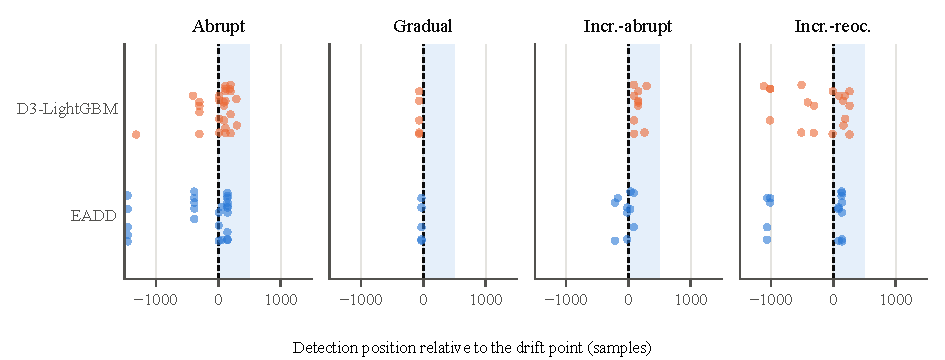
\includegraphics[width=\textwidth]{figures/detection_offsets.pdf}
    \caption[Detections around the annotated drift points]{Position of the EADD and D3-LightGBM detections relative to the nearest annotated drift point (dashed line) on the four INSECTS streams, all five seeds. A detection in the shaded tolerance window matches the drift point; any other detection is a false alarm.}
    \label{fig:offsets}
\end{figure}

\begin{figure}[!htbp]
    \centering
    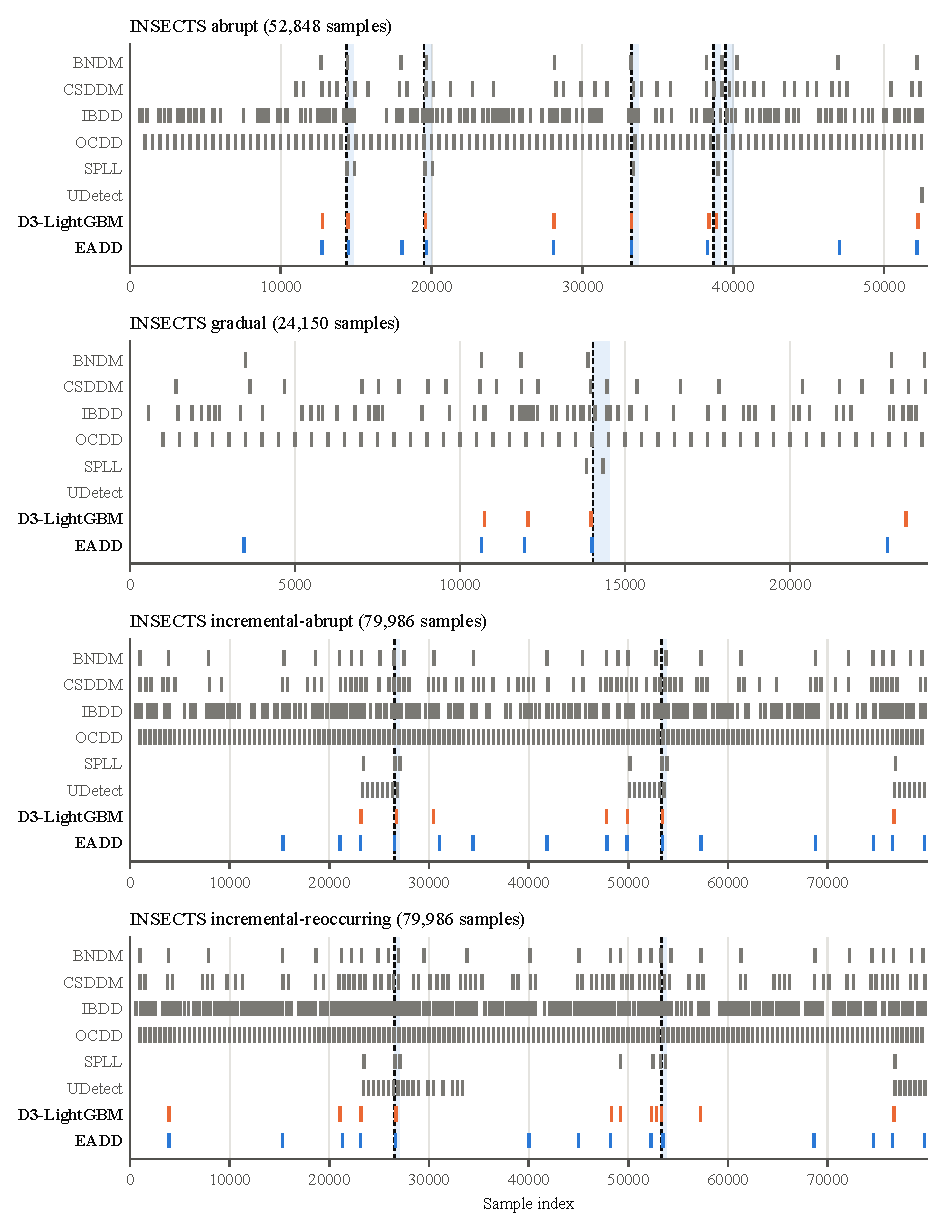
\includegraphics[width=\textwidth]{figures/detection_timeline.pdf}
    \caption[Detections on the annotated streams]{Detections of every detector on the four annotated INSECTS streams in the runs with seed 42. Dashed lines mark the annotated drift points and the shaded bands their tolerance windows of 500 samples.}
    \label{fig:timeline}
\end{figure}

Among the benchmark detectors, SPLL combined a high recall (0.95) and a mean MTD of 181 samples with the fewest false alarms (Experiment~2). CSDDM, IBDD and OCDD reached a recall of 1.00 on every stream, but with tens to hundreds of false alarms (Experiment~2). OCDD signalled drift exactly every 500 samples, the periodic behaviour that \citet{Lukats2024} filtered out because it requires no drift detector, and UDetect found few of the drift points (recall 0.38). BNDM had the lowest recall (0.35) and the longest MTD (440 samples) of all detectors. Its test has no random component, so its five seeds gave identical detections.

D3 checks the stream every 200 samples and EADD every 50 (Section~\ref{sec:baselines}). When EADD also checked every 200 samples, its mean recall rose to 0.80 and its MTD fell to 204 samples, because it raised fewer early alarms. These differences from D3-LightGBM were not significant (recall $p = 0.12$, MTD $p = 0.075$), and this was not the configuration specified in advance.

\section{Experiment 2: False Alarms (H2)}
\label{sec:exp2}

Table~\ref{tab:h2} reports the number of false alarms per run on the annotated streams.

\begin{table}[!htbp]
\centering
\caption[Experiment 2: false alarms on the annotated streams]{Experiment 2: Mean number of false alarms per run on the four annotated INSECTS streams (five seeds), and their sum over the streams. Prec.\ = precision, the share of all detections in the 20 runs that matched a drift point. Bold marks the best value in each column.}
\label{tab:h2}
\small
\begin{tabular}{l|cccc|c|c}
\hline
\textbf{Detector} & \textbf{Abrupt} & \textbf{Gradual} & \textbf{Incr.-abrupt} & \textbf{Incr.-reoc.} & \textbf{Total} & \textbf{Prec.} \\
\hline
\inputrows{tables/h2_rows.tex}
\hline
\end{tabular}
\end{table}

H2 is not supported. EADD raised more false alarms than D3-LightGBM on every stream, 8.9 against 5.6 per run on average (one-sided Mann--Whitney $p = 1.00$). The difference is significant in the opposite direction ($p < 0.001$) over the 20 runs, which are not independent (Section~\ref{sec:limitations}), and only 14\% of EADD's detections matched a drift point, against 25\% for D3-LightGBM. SPLL raised the fewest false alarms, 3.5 per run, while BNDM raised 18 and CSDDM, OCDD and IBDD between 53 and 273. Only 5\% of BNDM's detections matched a drift point. Only major transitions are annotated in the INSECTS streams, so some of these false alarms may be real changes, especially on the two incremental streams. This penalises the more sensitive and more frequently checking detectors more than the others, so part of EADD's excess of false alarms may come from real but unannotated changes.

\section{Experiment 3: Adaptive Sequential Permutation Test (H3)}
\label{sec:exp3}

Table~\ref{tab:h3} compares EADD with ASPT, with a full permutation test and without a test at the default threshold $\tau = 0.7$.

\begin{table}[!htbp]
\centering
\caption[Experiment 3: ASPT against a full permutation test]{Experiment 3: EADD with ASPT, with a full permutation test and without a permutation test at $\tau = 0.7$ on each annotated stream (five seeds) and over all 20 runs. Time = seconds spent in the detector per run, measured with one run at a time; Tests = permutation tests per run; Perm./test = permutations per test; Early = tests that stopped before 199 permutations (\%); Rej.\ = alarms rejected by the test (\%).}
\label{tab:h3}
\footnotesize
\setlength{\tabcolsep}{3pt}
\begin{tabular}{l|l|ccc|ccccc}
\hline
\textbf{Stream} & \textbf{Variant} & \textbf{Recall} & \textbf{MTD} & \textbf{FA} & \textbf{Time} & \textbf{Tests} & \textbf{Perm./test} & \textbf{Early} & \textbf{Rej.} \\
\hline
\inputrows{tables/h3_rows.tex}
\hline
\end{tabular}
\end{table}

H3 is supported. EADD with ASPT and EADD (full test) gave identical detections in all 20 runs, so their recall, MTD and false alarms are the same. Every ASPT test stopped after 20 permutations and confirmed the alarm, while the full test always drew 199. Measured with one run at a time, EADD with ASPT spent 112 seconds per run in the detector against 149 for EADD (full test), 25\% less, and it was faster in 20 of the 20 runs (one-sided paired Wilcoxon $p < 0.001$; Mann--Whitney $p = 0.022$). EADD (no test) took 107 seconds per run and gave the same detections, so at $\tau = 0.7$ the permutation test never changed a decision. H3a was therefore tested only in a setting where neither test rejected an alarm; the full test was not run at $\tau \leq 0.5$, where ASPT rejected 77\% to 98\% of the alarms, so whether its early stopping changes decisions there was not tested. Most of the runtime is spent training the classifier at every check, while a test ran at only about 10 of the roughly 1,100 checks of a run.

\subsection{Sensitivity to the AUC Threshold}
\label{sec:threshold}

Table~\ref{tab:threshold} repeats EADD with ASPT and EADD (no test) at lower thresholds, where the permutation test has to decide.

\begin{table}[!htbp]
\centering
\caption[Experiment 3: sensitivity to the AUC threshold]{Experiment 3: EADD with ASPT and without a test at thresholds $\tau = 0.3$ to $0.7$, averaged over 20 runs. Columns as in Table~\ref{tab:h3} without Tests, except that Time was measured with nine runs sharing the machine and is comparable only within this table; $p$ = one-sided Mann--Whitney test that the variant raises fewer false alarms than D3-LightGBM (5.6 per run).}
\label{tab:threshold}
\small
\setlength{\tabcolsep}{3.5pt}
\begin{tabular}{c|l|ccc|cccc|c}
\hline
$\boldsymbol{\tau}$ & \textbf{Variant} & \textbf{Recall} & \textbf{MTD} & \textbf{FA} & \textbf{Time} & \textbf{Perm./test} & \textbf{Early} & \textbf{Rej.} & $\boldsymbol{p}$ \\
\hline
\inputrows{tables/h3_threshold_rows.tex}
\hline
\end{tabular}
\end{table}

Without a test, lowering the threshold raised recall to 0.98 at $\tau = 0.3$ but also raised the false alarms to 87.8 per run. With ASPT, the test rejected 98\% of the alarms it examined at $\tau = 0.3$ and 77\% at $\tau = 0.5$, which reduced the false alarms to 16.8 and 16.7 per run (one-sided Mann--Whitney $p < 0.001$ and $p = 0.005$ against EADD (no test)). At $\tau = 0.5$, ASPT improved all three detection metrics over EADD (no test) (recall 0.67 vs.\ 0.60, MTD 264 vs.\ 307, false alarms 16.7 vs.\ 24.1), because fewer false alarms meant fewer resets of the reference window. ASPT stopped early in 96\% to 100\% of its tests at every threshold, but its runtime grew from 336 seconds per run at $\tau = 0.7$ to 886 seconds at $\tau = 0.3$, because it ran at most checks (935 tests per run at $\tau = 0.3$ against 10 at $\tau = 0.7$). No threshold gave EADD fewer false alarms than D3-LightGBM ($p \geq 0.99$ at every threshold). Figure~\ref{fig:threshold} shows these trade-offs.

\begin{figure}[!htbp]
    \centering
    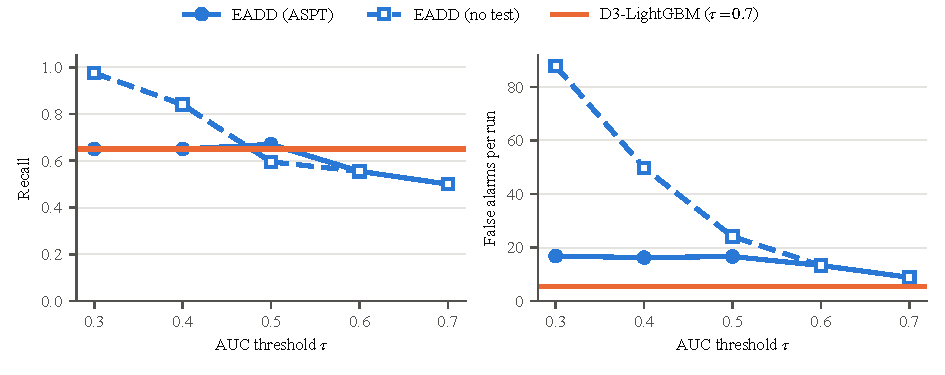
\includegraphics[width=\textwidth]{figures/threshold_sensitivity.pdf}
    \caption[Recall and false alarms against the AUC threshold]{Mean recall and false alarms per run of EADD with ASPT and without a test against the AUC threshold $\tau$ (20 runs per point). The horizontal line is D3-LightGBM at $\tau = 0.7$.}
    \label{fig:threshold}
\end{figure}

\section{Experiment 4: Streams without Annotated Drifts (RQ3)}
\label{sec:exp4}

Following \citet{Lukats2024}, Table~\ref{tab:e4-acc} reports the prequential accuracy of a Hoeffding tree that is reset at every detection, and Table~\ref{tab:e4-det} the number of detections and the lift-per-drift (Equation~\ref{eq:lpd}). The row ``No detector'' is a tree that is never reset.

\begin{table}[!htbp]
\centering
\caption[Experiment 4: classifier accuracy on the unannotated streams]{Experiment 4: Prequential accuracy (\%) of a Hoeffding tree reset at every detection on the nine unannotated streams, averaged over three seeds. Bold marks the best value in each column.}
\label{tab:e4-acc}
\small
\setlength{\tabcolsep}{2.5pt}
\begin{tabular}{l|ccccccccc|c}
\hline
\textbf{Detector} & \textbf{Elec.} & \textbf{Incr.} & \textbf{Lux.} & \textbf{NOAA} & \textbf{Outdoor} & \textbf{Ozone} & \textbf{Poker} & \textbf{Power} & \textbf{Rialto} & \textbf{Mean} \\
\hline
\inputrows{tables/e4_acc_rows.tex}
\hline
\end{tabular}
\end{table}

\begin{table}[!htbp]
\centering
\caption[Experiment 4: detections and lift-per-drift]{Experiment 4: Mean number of detections per stream, their total, and the mean lift-per-drift (LPD, percentage points of accuracy per detection) over the nine unannotated streams.}
\label{tab:e4-det}
\footnotesize
\setlength{\tabcolsep}{3pt}
\begin{tabular}{l|ccccccccc|cc}
\hline
\textbf{Detector} & \textbf{Elec.} & \textbf{Incr.} & \textbf{Lux.} & \textbf{NOAA} & \textbf{Outdoor} & \textbf{Ozone} & \textbf{Poker} & \textbf{Power} & \textbf{Rialto} & \textbf{Total} & \textbf{LPD} \\
\hline
\inputrows{tables/e4_det_rows.tex}
\hline
\end{tabular}
\end{table}

EADD and D3-LightGBM behaved almost identically on these streams. Their mean accuracies were 65.4\% and 65.7\% (two-sided Wilcoxon $p = 0.65$), they raised 477 and 512 detections in total, and their mean lift-per-drift was the highest of all detectors (4.2 and 3.9 percentage points per detection), but almost all of it comes from InsectsIncrementalBalanced, where each raised a single detection and the tree trained only on the first 1,000 samples reached 17.5\%; without that stream, BNDM, OCDD and SPLL had a higher lift-per-drift (0.97, 0.63 and 0.62 against 0.37 and 0.32). Resetting the classifier helped on Electricity, Outdoor Objects, PokerHand and RialtoBridge, where every detector except UDetect improved on the classifier that was never reset, and it hurt on Luxembourg and NOAA Weather. IBDD had the highest mean accuracy, 67.1\%, but it raised 9,411 detections, so its lift-per-drift was close to zero, and slightly negative because resetting lowered the accuracy on Luxembourg. BNDM raised 268 detections, with a mean accuracy of 65.1\% and a lift-per-drift of 1.7. UDetect raised no detection on these streams. As \citet{Lukats2024} observed, accuracy rewards frequent resets, so it does not show which detector finds the real changes.

\section{Summary of the Hypothesis Tests}

Table~\ref{tab:tests} summarises the significance tests. EADD did not detect the annotated drifts more completely or sooner than D3-LightGBM, and it raised more false alarms, so H1 and H2 are not supported. ASPT gave the same detections as a full permutation test in less time at $\tau = 0.7$, where neither test rejected an alarm, so H3 is supported.

\begin{table}[!htbp]
\centering
\caption[Summary of the hypothesis tests]{Summary of the hypothesis tests on the 20 runs of the annotated streams. EADD = mean of EADD with ASPT; Other = mean of D3-LightGBM or of EADD (full test); MW = one-sided Mann--Whitney U test; W = one-sided paired Wilcoxon signed-rank test.}
\label{tab:tests}
\small
\setlength{\tabcolsep}{3.5pt}
\begin{tabular}{p{4.7cm}|cc|cc|l}
\hline
\textbf{Hypothesis} & \textbf{EADD} & \textbf{Other} & \textbf{$p$ (MW)} & \textbf{$p$ (W)} & \textbf{Result} \\
\hline
H1a: higher recall than D3-LightGBM & 0.50 & 0.65 & 0.90 & 0.96 & Not supported \\
H1b: lower MTD than D3-LightGBM & 302 & 279 & 0.78 & 0.85 & Not supported \\
H2: fewer false alarms than D3-LightGBM & 8.9 & 5.6 & 1.00 & 1.00 & Not supported \\
H3a: same detections as the full test & \multicolumn{4}{c|}{identical in 20 of 20 runs} & Supported \\
H3b: lower runtime than the full test (s) & 112 & 149 & 0.022 & $<$0.001 & Supported \\
\hline
\end{tabular}
\end{table}


\chapter{Discussion} \label{chap:discussion}

This chapter interprets the results of Chapter~\ref{chap:results}, answers the research questions, and relates the findings to the studies reviewed in Chapter~\ref{chap:literature}.

\section{Answers to the Research Questions}

\subsection{RQ1: Detection and False Alarms against D3}

\textit{Does EADD detect annotated drifts in real-world data streams more completely and sooner than D3, and does it raise fewer false alarms?}

No. When D3 used the same LightGBM classifier and the same window sizes as EADD, EADD had a lower recall (0.50 vs.\ 0.65), a higher MTD (302 vs.\ 279 samples) and more false alarms (8.9 vs.\ 5.6 per run) on the four annotated INSECTS streams. The difference in false alarms was significant in favour of D3-LightGBM, and the differences in recall and MTD were not significant in favour of EADD.

Two features of the evaluation explain much of the recall gap. First, EADD often signalled a drift shortly before the annotated point, which the matching rule counts as a false alarm followed by a missed drift. When detections up to 500 samples before an annotated point were also accepted, both detectors reached a recall of 0.95, while EADD still raised more false alarms (8.1 vs.\ 5.3 per run). Second, EADD checks the stream every 50 samples, four times as often as D3. More checks give more chances for an early or false alarm, and each alarm leaves EADD unable to signal for about 500 samples while its windows refill. When EADD checked every 200 samples, its recall and MTD were better than those of D3-LightGBM, although not significantly, while it still raised more false alarms (7.3 vs.\ 5.6 per run). Neither observation was part of the planned comparison, so they do not change the test results, but they show that the comparison is sensitive to the check interval and to the exact position of the annotated drift points.

These results differ from the earlier evaluation of EADD, in which EADD detected the gradual and incremental synthetic drifts that D3 missed and raised fewer false alarms on stable synthetic streams. That evaluation compared EADD with D3 using logistic regression and smaller windows, used synthetic data, and computed the MTD only over the drifts that a detector found. With these differences removed, the advantage of EADD on real data was not confirmed.

\subsection{RQ2: The Adaptive Sequential Permutation Test}

\textit{Does the sequential stopping rule of ASPT make the permutation test faster without degrading detection, and how does the AUC threshold affect EADD?}

Yes for the first part. At the default threshold, ASPT gave exactly the same detections as a full permutation test in every run and stopped every test after 20 of 199 permutations, which reduced the detector's runtime by 25\%. At this threshold the test never changed a decision, because an AUC above 0.7 was always far beyond the AUCs obtained with shuffled labels.

The threshold sensitivity shows when the test matters. At $\tau = 0.5$ and below, most alarms were rejected by ASPT, which reduced the false alarms by 31\% to 81\% compared with EADD without a test, and at $\tau = 0.5$ it also improved recall and MTD. ASPT still stopped early in at least 96\% of its tests. The cost is runtime, which more than doubled at $\tau = 0.3$, and even with ASPT, EADD raised more false alarms than D3-LightGBM at every threshold.

\subsection{RQ3: Streams without Annotated Drifts}

\textit{How do EADD and the other detectors behave on real-world streams without annotated drift points?}

EADD and D3-LightGBM behaved almost identically: their classifier accuracies, numbers of detections and lift-per-drift values were close, and the accuracies did not differ significantly. Resetting a classifier at the detections improved accuracy on four streams and reduced it on two. The detector with the most detections, IBDD, had the highest accuracy but a negative lift-per-drift. These proxy metrics therefore do not separate EADD from D3.

\section{Relation to Previous Studies}

\citet{Lukats2024} found D3 to be one of the strongest unsupervised detectors, with the best mean time ratio on INSECTS Abrupt. The results agree that D3, here with a LightGBM classifier, is a strong baseline: it matched or exceeded EADD on every metric averaged over the annotated streams, and EADD was better only on Incr.-reoc. \citet{Lukats2024} also reported that the observed sample size strongly influences the detectors and that some configurations signal drift periodically. Both effects appeared here: OCDD signalled drift exactly every 500 samples, and the recall of CSDDM, IBDD and OCDD came with tens to hundreds of false alarms. BNDM, which signalled drift periodically with few observed samples in their study, was not periodic with 500 samples per window, but it had the lowest mean recall (0.35). SPLL, which \citet{Lukats2024} ranked third under the mean time ratio, behind D3 and close to BNDM, combined a high recall with the fewest false alarms on these four streams, which shows how much the ranking of detectors depends on the metric and on the streams.

The behaviour of ASPT follows from the theory of the classifier two-sample test \citep{LopezPazOquab2017}. Under the null hypothesis, the held-out accuracy of the classifier concentrates near 0.5 \citep{LopezPazOquab2017}, and the AUC of a classifier trained on shuffled labels likewise concentrates near 0.5, so an AUC above 0.7 is far in the tail and a permutation test confirms it; sequential stopping then saves most of the permutations. When the threshold is close to 0.5, the test decides, but because a test is run at every check, the false alarm rate over a whole stream is not controlled. Anytime-valid tests such as E-C2ST \citep{EC2ST2024} address this problem.

The accuracy-based evaluation of the unannotated streams reproduced the concern of \citet{Lukats2024} that classifier accuracy rewards frequent resets: IBDD had the highest accuracy with more than 9,000 detections. Lift-per-drift corrects for this, but on these streams it did not distinguish EADD from D3.

\section{Practical Implementation Considerations}

\subsection{Check Interval, Threshold and Resets}

The experiments show three practical points for discriminative detectors. First, every detection resets the windows, after which the detector cannot signal for about the length of its windows. A false alarm shortly before a real drift can therefore cause the real drift to be missed, so a detector that checks often should also be selective. Second, a threshold of 0.7 made the permutation test unnecessary in these experiments; a lower threshold needs a test to keep the false alarms down and costs more computation. Third, the check interval affected the results more than the significance test did, and the window sizes, which were not varied here, may matter as well; both should be chosen for the stream at hand.

\subsection{Proposed MLOps Deployment Architecture}

To move EADD from an offline experiment to a production service, it would be integrated into a machine learning operations (MLOps) architecture as a separate monitoring service:

\begin{itemize}
    \item \textbf{Data Ingestion Layer (e.g., Apache Kafka):} streams the incoming feature data ($W_{cur}$) to the monitoring service.
    \item \textbf{EADD Monitoring Service:} a container that runs the LightGBM discriminator, the permutation test and the SHAP explainer, and keeps the reservoir sample ($W_{ref}$) in an in-memory store (e.g., Redis).
    \item \textbf{Orchestration and Model Registry (e.g., Apache Airflow, MLflow):} receives a drift report with the AUC, the p-value, $H_{\text{pred}}$ and the feature ranking, and either triggers retraining of the deployed model or alerts the engineers responsible for the top-ranked features.
\end{itemize}

This architecture keeps the cost of the discriminator and the permutation test away from the inference path of the deployed model.

\section{Limitations and Threats to Validity}
\label{sec:limitations}

\textbf{Few Annotated Drifts:} The four annotated streams contain ten drift points, and only major transitions are annotated. Recall and false alarms therefore rest on few events, and some false alarms on the incremental streams may be real changes.

\textbf{Matching Rule:} A detection counts only if it occurs within 500 samples after an annotated point. EADD's recall depended strongly on this choice, because many of its detections came shortly before the annotated points.

\textbf{Dependent Runs:} The five seeds of a stream share the same data, so the 20 runs of a detector are not independent samples. The tests treat them as independent, which overstates the evidence for any difference.

\textbf{Check Grid:} All runs start at sample 0, so each detector checks at the same positions in every seed, and whether a detection falls just before or just after an annotated point depends on this grid. In an additional run that started the five seeds at samples 0, 40, 80, 120 and 160, the recall of D3-LightGBM rose from 0.65 to 0.82 and that of EADD from 0.50 to 0.53, so the size of the recall difference depends on the grid, although its direction did not change.

\textbf{Post-hoc Analyses:} The explanations of the recall gap and the threshold sensitivity analysis use the same 20 runs as the hypothesis tests, so they were not validated on held-out streams.

\textbf{Check Interval and Cross-Validation:} D3 checks every 200 samples and estimates the AUC with 2-fold cross-validation, while EADD checks every 50 samples and uses 5-fold cross-validation; both are part of their designs but remain differences between them. EADD checking every 200 samples was reported as an additional run.

\textbf{Default Configurations:} All detectors used one configuration with 500 observed samples, while \citet{Lukats2024} tested many configurations per detector. Other configurations may change the ranking.

\textbf{Approximate Permutation Test:} ASPT's stopping rules raise its Type~I error from 0.045 to 0.059 at $\alpha = 0.05$ in simulation, and the permuted AUCs use 2-fold cross-validation while the observed AUC uses 5-fold cross-validation. EADD also tests at every check without correcting for the number of tests, and the permutation test assumes exchangeable samples, which autocorrelated streams violate.

\textbf{Reference/Current Overlap:} In the implementation, a new sample can enter the reservoir while it is still in the current window, so some samples, many of them shortly after the reference window refills, appear in both windows with opposite labels. This lowers the AUC and may affect EADD's recall and false alarms.

\textbf{Covariate Drift Only:} EADD detects changes in $P(X)$ and cannot detect concept drift that leaves $P(X)$ unchanged \citep{Gama2014, Webb2016}.

\textbf{Unevaluated Components:} The prediction entropy $H_{\text{pred}}$ and the TreeSHAP feature ranking are reported by EADD but were not evaluated. SHAP explanations are also exploratory rather than causal \citep{CausalDrift2025}.

\textbf{Difference from the Conference Paper:} The conference version of this work used synthetic streams, D3 with logistic regression and smaller windows, a single real-world run, and the Drift Severity Index. Its conclusions about EADD's advantage over D3 are not confirmed by the evaluation in this thesis.

\textbf{Adversarial Vulnerability:} \citet{AdvAttackDrift2024} showed that discriminative drift detectors can be evaded by adversarial data streams, and EADD shares this weakness.

\section{Chapter Summary}

With the classifier and the window sizes matched, EADD did not outperform D3-LightGBM on the annotated real-world streams: its recall was lower, its detection delay longer and its false alarms more frequent, so H1 and H2 are not supported. Additional analyses on the same streams, not part of the planned comparison, suggest that much of the recall gap came from EADD signalling shortly before the annotated drift points and from its more frequent checks. ASPT gave the same detections as a full permutation test in less time, which supports H3, and at low thresholds it rejected most alarms and reduced the false alarms substantially. On the unannotated streams, EADD and D3-LightGBM behaved almost identically, and their accuracies did not differ significantly.

\chapter{Conclusion and Recommendations} \label{chap:conclusion}

\section{Summary of Findings}

This thesis investigated adversarial validation, the classifier two-sample test, as a technique for unsupervised feature drift detection. It proposed EADD, which extends the discriminative approach of D3 \citep{Gozuacik2019} with a long-memory reference window, a permutation test with sequential stopping, prediction entropy monitoring and a feature ranking. The contributions are the following:

\begin{enumerate}
    \item An integrated framework that combines a classifier two-sample test \citep{LopezPazOquab2017}, a reservoir-sampled reference window \citep{Vitter1985}, prediction entropy monitoring and an adaptive sequential permutation test, and that ranks the features behind each confirmed drift.
    \item An adaptive sequential permutation test (ASPT) that adds a sequential stopping rule, motivated by \citet{Gandy2009}, to the classifier two-sample test.
    \item A comparison of EADD with D3 and six other unsupervised detectors on thirteen real-world streams, with D3 using the same classifier and window sizes as EADD and the differences between EADD and D3 tested for significance.
\end{enumerate}

On four annotated INSECTS streams, EADD had a lower recall (0.50 vs.\ 0.65) and a higher MTD (302 vs.\ 279 samples) than D3-LightGBM, so H1 is not supported. EADD also raised more false alarms (8.9 vs.\ 5.6 per run), and this difference was significant in favour of D3-LightGBM, so H2 is not supported.

At the default threshold of 0.7, where every test confirmed its alarm, ASPT gave the same detections as a full permutation test in all 20 runs with 25\% less runtime, so H3 is supported. Whether ASPT matches a full test at thresholds where the test rejects alarms was not tested, and a simulation shows that the sequential stopping rule raises the Type~I error of a single test from 0.045 to 0.059 at $\alpha = 0.05$. At thresholds of 0.5 and below, ASPT reduced the false alarms of EADD by 31\% to 81\% compared with no test.

Among the six benchmark detectors, SPLL, a density-based statistical detector, had a higher recall (0.95), a shorter MTD (181 samples) and fewer false alarms (3.5 per run) than both EADD and D3-LightGBM, so the discriminative detectors did not detect drift earlier than this statistical method. CSDDM, IBDD and OCDD reached full recall only with tens to hundreds of false alarms.

On the nine unannotated streams, EADD and D3-LightGBM gave almost the same classifier accuracy (65.4\% vs.\ 65.7\%) and lift-per-drift.

\section{Limitations}

The main limitations, discussed in Section~\ref{sec:limitations}, are the small number of annotated drift points, the dependence of the results on the matching rule and the check interval, the use of one configuration per detector, and the dependence between runs on the same stream. ASPT is not an exact level-$\alpha$ test, the error rate over a whole stream is not controlled, and the prediction entropy and the feature ranking were not evaluated.

\section{Recommendations for Application}

The results lead to the following recommendations for practitioners who deploy discriminative drift detectors:

\textbf{Start from D3 with a Strong Classifier:} On the annotated real-world streams, D3 with a LightGBM classifier had a higher mean recall, a lower mean MTD and significantly fewer false alarms than EADD. It is a strong default for unsupervised feature drift detection.

\textbf{Match the Check Interval to the Windows:} Every detection resets the windows. Checking very often gives more chances for early or false alarms, each of which leaves the detector unable to signal for about the length of its windows.

\textbf{Use a Permutation Test Only with a Low Threshold:} At an AUC threshold of 0.7, the permutation test never changed a decision. With a lower threshold, a test is needed to keep the false alarms down, and sequential stopping keeps most tests to 10 to 20 permutations.

\textbf{Evaluate on Annotated Real Data and Count Missed Drifts:} Synthetic streams and an MTD computed only over the drifts that a detector finds can favour one detector over another. Evaluations should use annotated real-world streams where possible and report recall, MTD with missed drifts counted, and false alarms together.

\textbf{Treat the Feature Ranking as a Lead:} The TreeSHAP ranking points to the features that separate the two windows. Because its accuracy has not been evaluated and SHAP explanations are exploratory rather than causal \citep{CausalDrift2025}, it should be treated as a lead for investigation rather than as a diagnosis. In regulated settings, where rules such as the EU GDPR restrict automated decision-making and give individuals a right to an explanation \citep{GoodmanFlaxman2017}, it can also document which features changed before each update.

\section{Suggestions for Future Research}

Based on the findings, future research could pursue the following directions:

\begin{enumerate}
    \item \textbf{Selective Resets:} Keeping the reference window after an alarm that is not confirmed by later checks, so that an early or false alarm does not make the detector blind to a real drift that follows.
    \item \textbf{Anytime-Valid Testing:} Replacing the per-check permutation p-value with e-values \citep{EC2ST2024} to control the false alarm rate over a whole stream, and using a sequential test with exact level \citep{BesagClifford1991}.
    \item \textbf{More Annotated Streams and Configurations:} Evaluating the detectors on more real-world streams with annotated drift points, with several configurations per detector as in \citet{Lukats2024}, and with matching rules that accept detections close to an annotated point.
    \item \textbf{Evaluating the Feature Ranking and $H_{\text{pred}}$:} Measuring how accurately the TreeSHAP ranking identifies drifting features, and whether $H_{\text{pred}}$ gives earlier warnings than the AUC.
    \item \textbf{Covariate and Concept Drift Decomposition:} Integrating the decomposition of \citet{HDPD2024} to separate $P(X)$ shifts from $P(y|X)$ shifts when delayed labels become available.
    \item \textbf{Adversarial Robustness:} Developing defences against adversarial drift evasion attacks \citep{AdvAttackDrift2024}.
\end{enumerate}

\section{Concluding Remarks}

This thesis studied adversarial validation as a technique for feature drift detection and proposed EADD, an integrated framework that combines established methods: the classifier two-sample test \citep{LopezPazOquab2017}, reservoir sampling \citep{Vitter1985}, sequential stopping of Monte Carlo tests \citep{Gandy2009} and TreeSHAP \citep{Lundberg2017, LundbergInteraction2020}. When D3 was given the same classifier and window sizes, EADD did not outperform it on annotated real-world streams, and the earlier advantage of EADD did not hold under this fairer comparison. At the default threshold, where every test confirmed its alarm, the sequential permutation test gave the same detections as a full permutation test in less time, and with a low threshold it reduced false alarms compared with no test; whether it matches a full test where the test rejects alarms was not tested. The main lesson is that the check interval and the evaluation protocol of a discriminative drift detector affected the results more than its significance test, which at the default threshold never changed a decision, and that claims about such detectors should be tested on annotated real-world data with the confounding choices held equal.


\bibliographystyle{unsrtnat}
\bibliography{references}

\appendices
\chapter{Implementation Details} \label{app:implementation}

This appendix lists the hyperparameters and settings of EADD used in the final test, so that the runs can be reproduced.

\section{Adversarial Classifier (LightGBM)}
The adversarial classifier uses LightGBM \citep{Ke2017} with the configuration in Table~\ref{tab:lgbm-params}. D3-LightGBM, the version of D3 used in the experiments, uses the same configuration.

\begin{table}[!htbp]
\centering
\caption{LightGBM hyperparameters of EADD and D3-LightGBM.}\label{tab:lgbm-params}
\small
\begin{tabular}{ll}
\toprule
Parameter & Value \\
\midrule
Boosting type & gbdt \\
Number of trees & 50 \\
Learning rate & 0.1 \\
Maximum depth & $-1$ (no limit) \\
Maximum leaves per tree & 31 \\
Objective & binary classification \\
Metric & default (binary log-loss; not used, no early stopping) \\
Verbosity & $-1$ \\
Threads & 1 (\texttt{n\_jobs=1}) \\
\bottomrule
\end{tabular}
\end{table}

\section{Windowing, Testing and Attribution}
Table~\ref{tab:eadd-settings} lists the remaining settings of EADD in the final test, with the option of \nolinkurl{detectors/eadd.py} that selects each.

\begin{table}[!htbp]
\centering
\caption{Windowing, test and attribution settings of EADD in the final test.}\label{tab:eadd-settings}
\small
\begin{tabular}{>{\raggedright\arraybackslash}p{3.3cm}>{\raggedright\arraybackslash}p{10.1cm}}
\toprule
Setting & Value \\
\midrule
Reference window & 500 samples, a uniform random sample of all samples since the last alarm, maintained with reservoir sampling (Algorithm~R) \citep{Vitter1985}; a sample is offered to the reservoir only when it leaves the current window. \newline\mbox{\footnotesize\texttt{reservoir\_after\_current=True}} \\
\addlinespace
Current window & the newest 200 samples \\
\addlinespace
Check interval & every 50 samples; each seed starts the stream at a random offset of 0--49 samples \\
\addlinespace
After an alarm & the reference is replaced by the 200 samples of the current window and filled up to 500 with the next 300 samples; the current window is emptied and refilled, so the next check is made 500 samples after the alarm; the history of the permutation test restarts from the same 200 samples \\
\addlinespace
Alarm rule & out-of-fold AUC (stratified 5-fold cross-validation) at least $\tau = 0.7$ and rejection by ASPT at $\alpha = 0.05$ \\
\addlinespace
Null distribution & AUCs of earlier 200-sample windows of the same stream against the reference, one window start every 10 samples, from at most the newest 5,000 samples since the last alarm, drawn in random order; each null AUC uses the same 5-fold cross-validation as the observed AUC. \newline\mbox{\footnotesize\texttt{null="history"}, \texttt{history\_stride=10},}\newline\mbox{\footnotesize\texttt{perm\_n\_folds=None}} \\
\addlinespace
ASPT & at most 199 draws, $B_{\min} = 10$; early rejection when no draw among the first $i$ reaches the observed AUC and $1/(i+1) \leq \alpha/3$; early acceptance when, after at least $B_{\min}$ draws, more than a fraction $2\alpha$ of them reach it; otherwise rejection when $p \leq 2\alpha/3$. \newline\mbox{\footnotesize\texttt{aspt\_alpha\_split=1/3}} \\
\addlinespace
Feature attribution & TreeSHAP on a LightGBM model with the settings of Table~\ref{tab:lgbm-params}, trained on $W_{\mathrm{ref}} \cup W_{\mathrm{cur}}$ after each alarm; features ranked by normalised mean absolute SHAP value \\
\bottomrule
\end{tabular}
\end{table}


\biography
% \ps@headings sets \topskip to 0pt, so the \clearpage at the end of the document
% would ship out a blank page after the Biography.
\setlength{\topskip}{1pt}

\end{document}
